\section{Exeperiments and Results}
\label{sec:benchmark}

In this section, we demonstrate the efficacy of our approaches via a set of benchmarks.

\subsection{Experiment system}
\label{sec:system}

Mira \cite{Chen:BGQ}, with 48 compute racks (48K nodes and 768K cores) at the ALCF, provides 10 PFlops theoretical peak performance. Each node has a 16-core processor and 16 GB of memory.

The interprocess communications of Blue Gene/Q travel on a 5D torus network both for point-to-point and for collective communications. This 5D torus interconnects a compute node with its 10 neighbors at 2 GB/s theoretical peak over each link in each direction, making a total of 40 GB/s bandwidth in both directions for a single compute node. Because of packet and protocol overheads, however, only up to 90\% of the raw data rate (1.8 GB/s) is available for user data. The machine can be partitioned into non-overlapping rectangular submachines; these submachines do not interfere with each other except for I/O nodes and the corresponding storage system.

For interconnect network traffic, BG/Q supports both deterministic and dynamic routing \cite{Chen:BGQ}. In the dynamic routing, messages in different message size ranges can be routed differently. However, within a given message size range, routing is always the same, and its path is known before it is routed. These are the default routing algorithms and cannot be changed during run time. The BG/Q supercomputer uses single-path data routing, for sending/receiving a message only one link of the ten available is used. The details of routing can be found in \cite{Chen:BGQ}.

PAMI is a low-level communication library for BG/Q \cite{PAMI:Kumar}. PAMI provides low-overhead communication by using various techniques such as accelerating communication using threads, scalable atomic primitives, and lockless algorithms to increase the messaging rate. Since MPI is implemented on top of PAMI, direct use of PAMI would provide higher messaging rates as well as lower latencies in comparison with MPI.




\subsection{Experiment setup}

We carried our experiments on Mira, a Blue Gene/Q supercomputer. In our experiments, we varied paritition size from 512 nodes up to 8012 nodes. The experiments involved a subset or entire set of nodes for each partition. The number sources and destinations and distance between them are also varied depending on each experiment. We also varied the data sizes to be exchanged to find the effective data size. Pairs of sources and destinations are randomized to show the efficacy of our works. We varied the number of paths fed into solvers to measure the effectiveness of number of paths to throughput. A similar benchmark with various max load is done for heuristic approach. Our experiments covered 3 communication patterns: disjoint, overlap and subset. For the commnication patterns, we demonstrated the efficacy of our algorithms in comparions with MPI\_Alltoallv.

For searching optimal paths, we AMPL and its solvers \cite{AMPL} for modleing our problem and to find solutions for optimal data movement.

\subsection{MPI Paths Reconstruction}

In our experiment, we need to measure not only the performance of MPI routines but also loads on physical links and number of hops of path that MPI takes to move data from a set of sources to a set of destination. The load and hops informaiton can reveal insight of performance difference between MPI and our framework OPTIQ. Thus reconstructing MPI's paths is necessary to get load and hops information.

We reconstruct MPI's paths based on our understanding of default routing algorithms described in \cite{Chen:BGQ}. For each pair of source and destination, we start at a source node and follow the rules of the routing algorithm to move data from the source node to its destination. We then record paths for all the pairs and use them to calculate load and number of hops. 

\subsection{Communication Patterns}
In this paper we demostrate data movement performance of our OPTIQ framework and existing MPI's routines on the following communication patters:

\begin{figure}[ht]
\vspace{-0.1in}
\centering
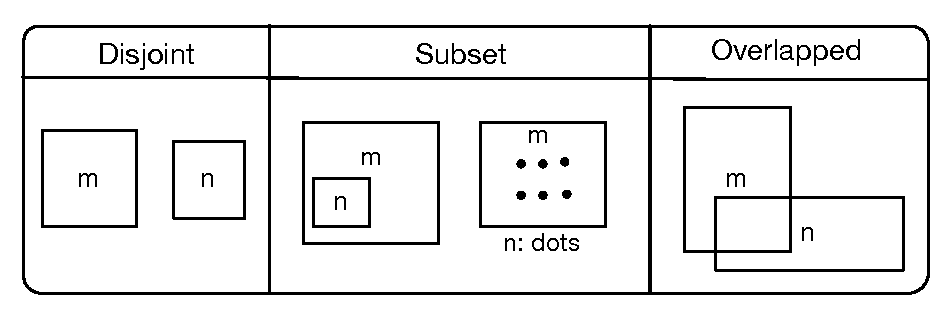
\includegraphics[scale=0.55]{figures/patterns.pdf}
\vspace{-0.1in}
\caption{Communication patterns}
\vspace{-0.1in}
\label{fig:patterns}
\end{figure}

\begin{itemize}
\item Disjoint sets: is many-to-many communication pattern where the sources and destinations are separated. It is a typical pattern in many applications.
\item Overlap: is a many-to-many pattern that sources and destinations are overlapped sets. CESM uses this communication patterns for its coupling communications.
\item Subset: is a many-to-many pattern that sources or destinations are subset of the other. The patterns can be found CESM or in I/O aggregation.
\end{itemize}

We carried a set of experiments to study the system's behavior in various patterns and demontrate throughput improvement.

\subsection{Experimental results}

In the experiments, we collected the throughput, total number fo paths, maximum and average values for number of paths per job, hopbytes (total bytes x number of hops) per path, number of copies per paths, number of paths per link and total amount of data per link while varying communication patterns, source destination pairing, distance and sizes of sources and destinations, partition sizes, message sizes, chunk size.
In the next subsections, we go into each communication and study in details the system's behaviors and performance.

\subsubsection{Varying partition, source and destination sizes, keeping the same sources/destination ratio}

\begin{figure*}[!htbp]
        \centering
        \begin{subfigure}[b]{0.32\textwidth}
                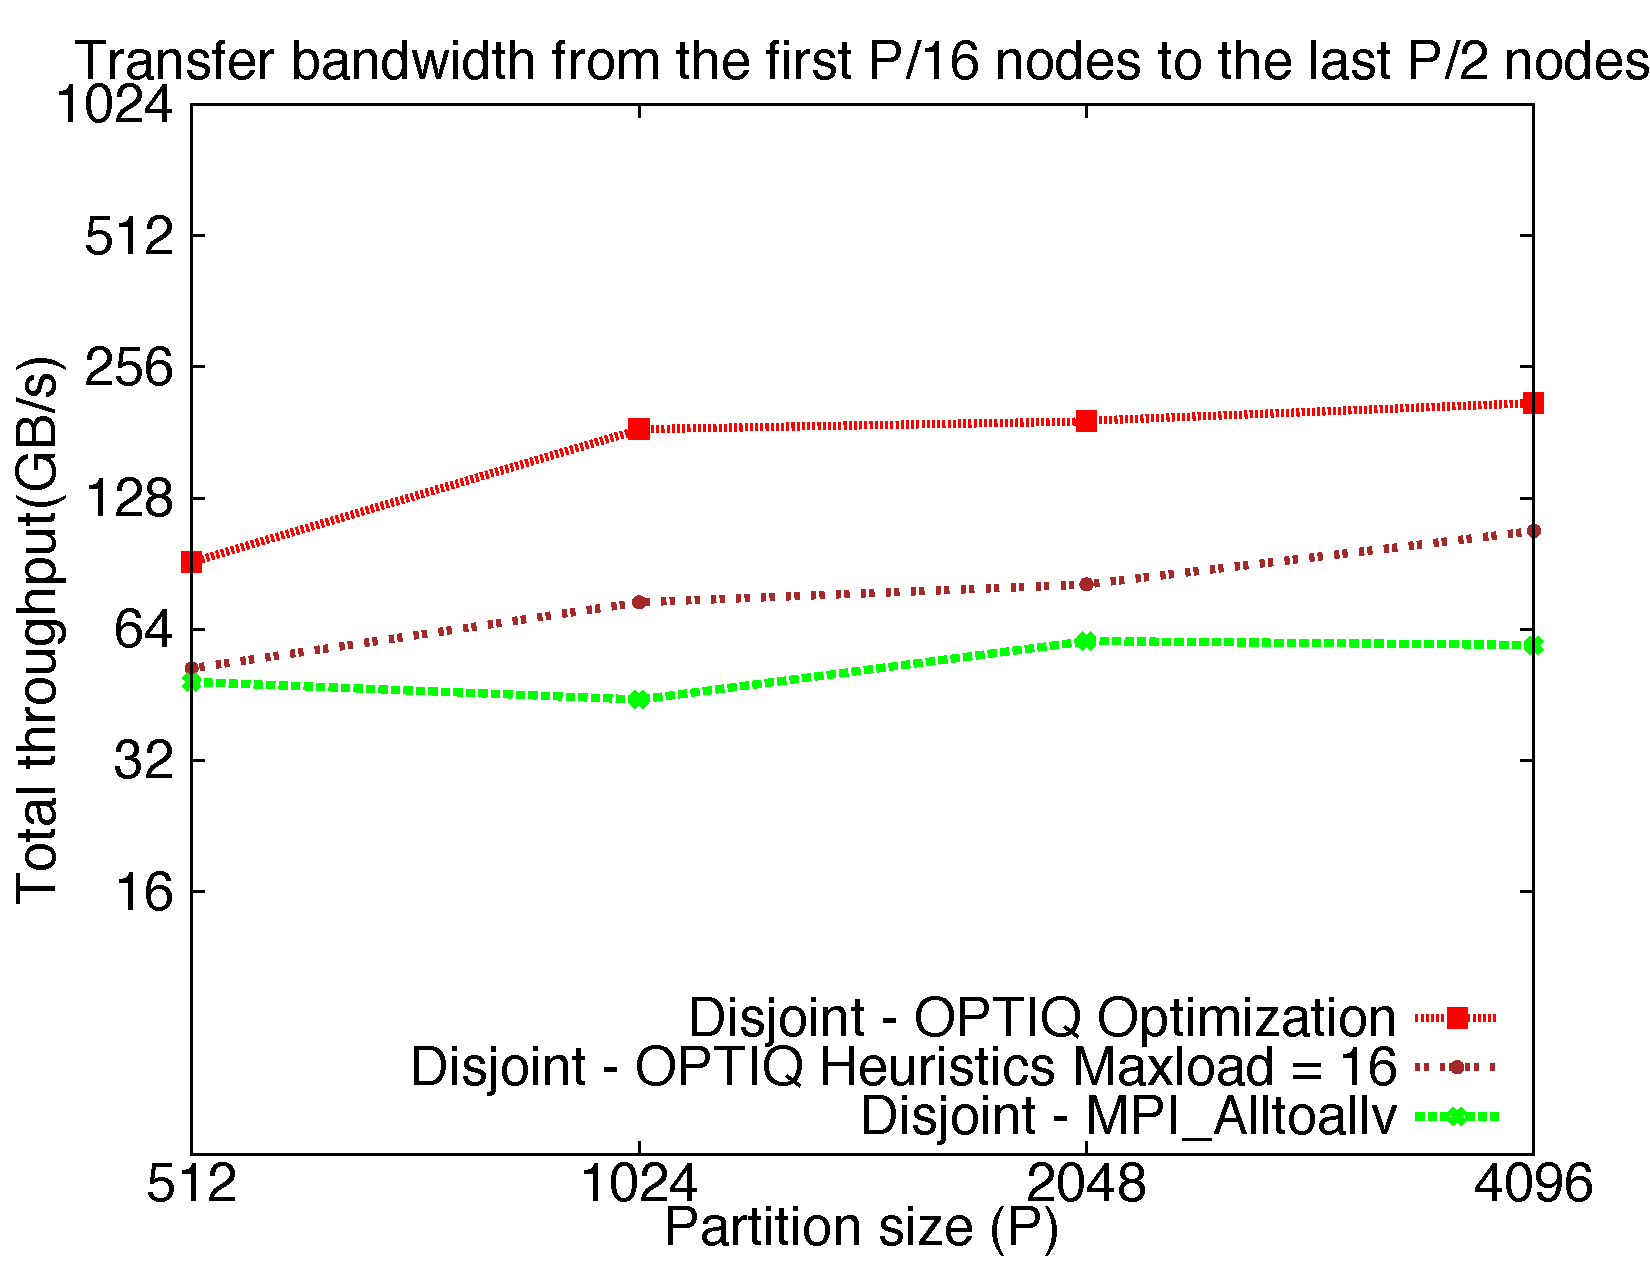
\includegraphics[width=\textwidth]{figures/constantr_3.pdf}
                \caption{Disjoint}
                \label{fig:constantr_3}
        \end{subfigure}%
        ~ %add desired spacing between images, e. g. ~, \quad, \qquad, \hfill etc.
          %(or a blank line to force the subfigure onto a new line)
        \begin{subfigure}[b]{0.32\textwidth}
                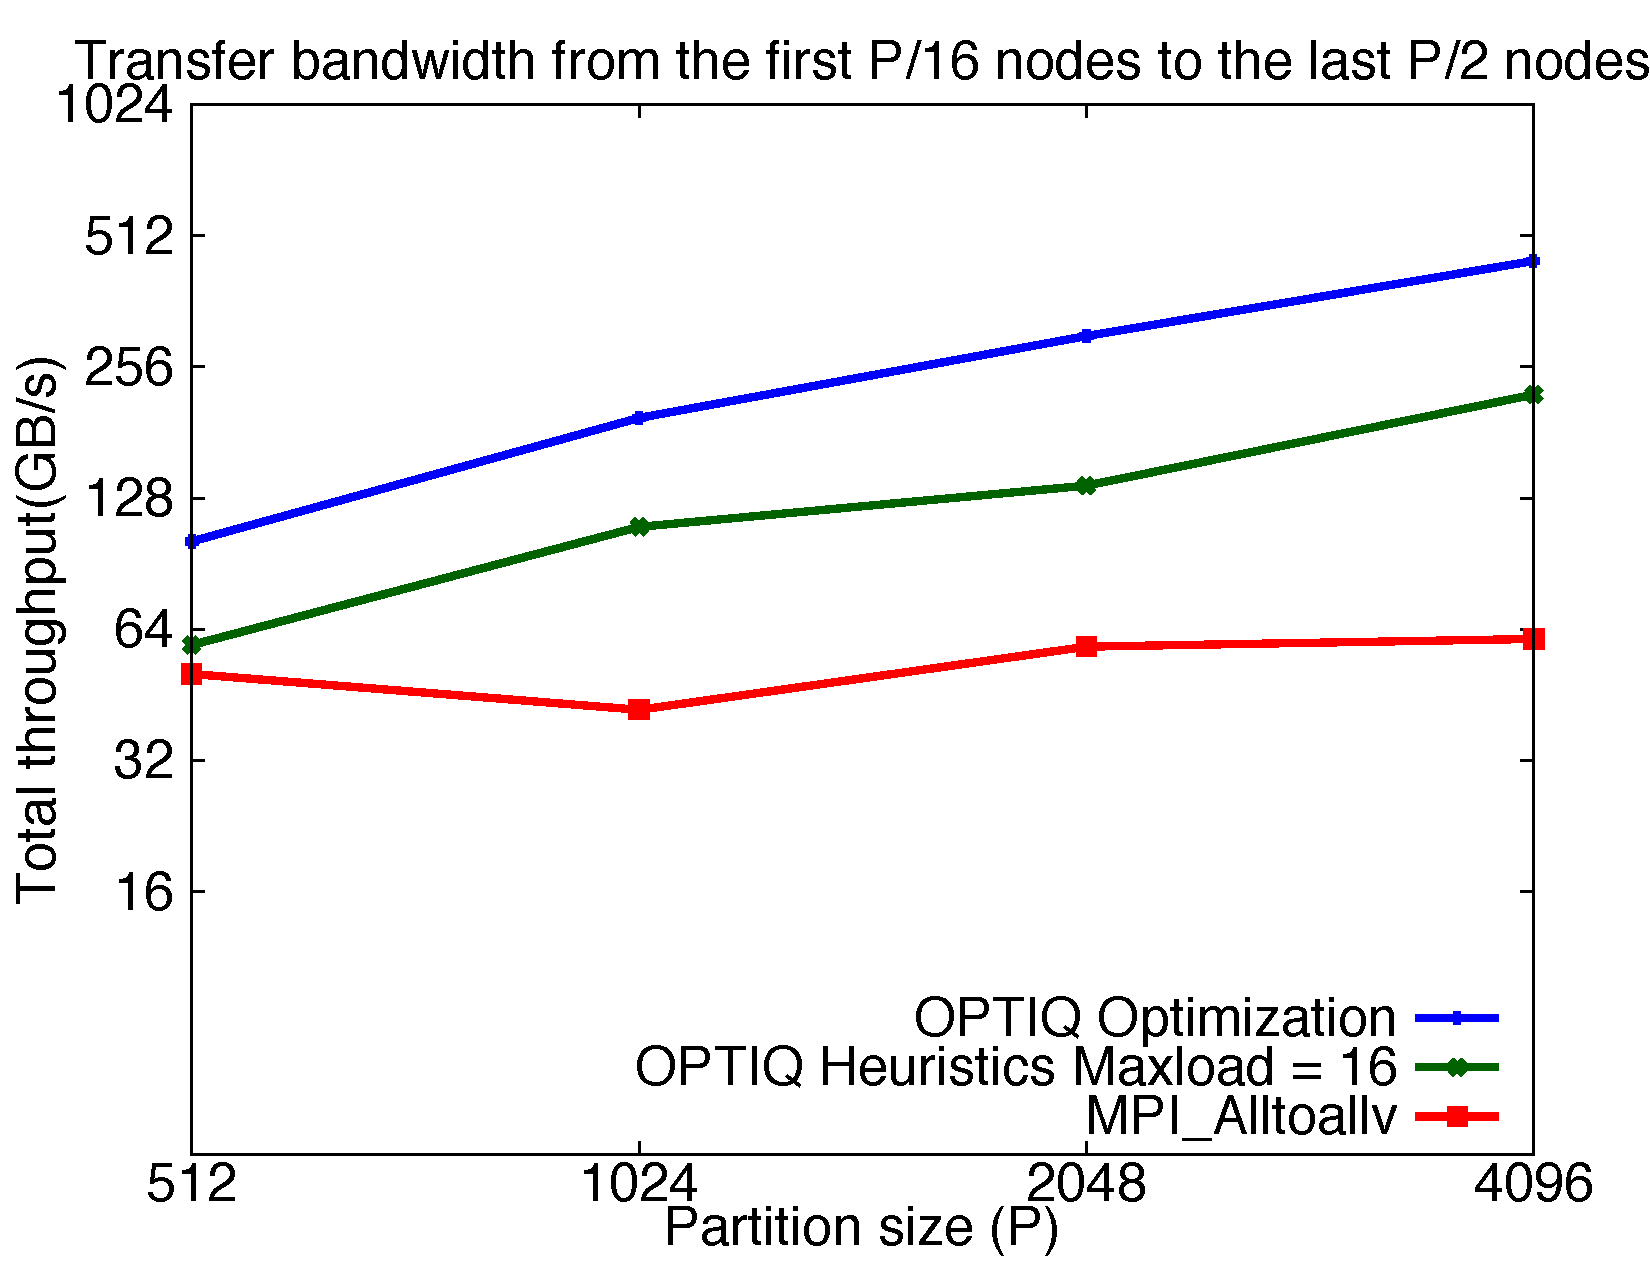
\includegraphics[width=\textwidth]{figures/constantr_27}
                \caption{Overlap}
                \label{fig:constantr_27}
        \end{subfigure}
        ~ %add desired spacing between images, e. g. ~, \quad, \qquad, \hfill etc.
          %(or a blank line to force the subfigure onto a new line)
        \begin{subfigure}[b]{0.32\textwidth}
                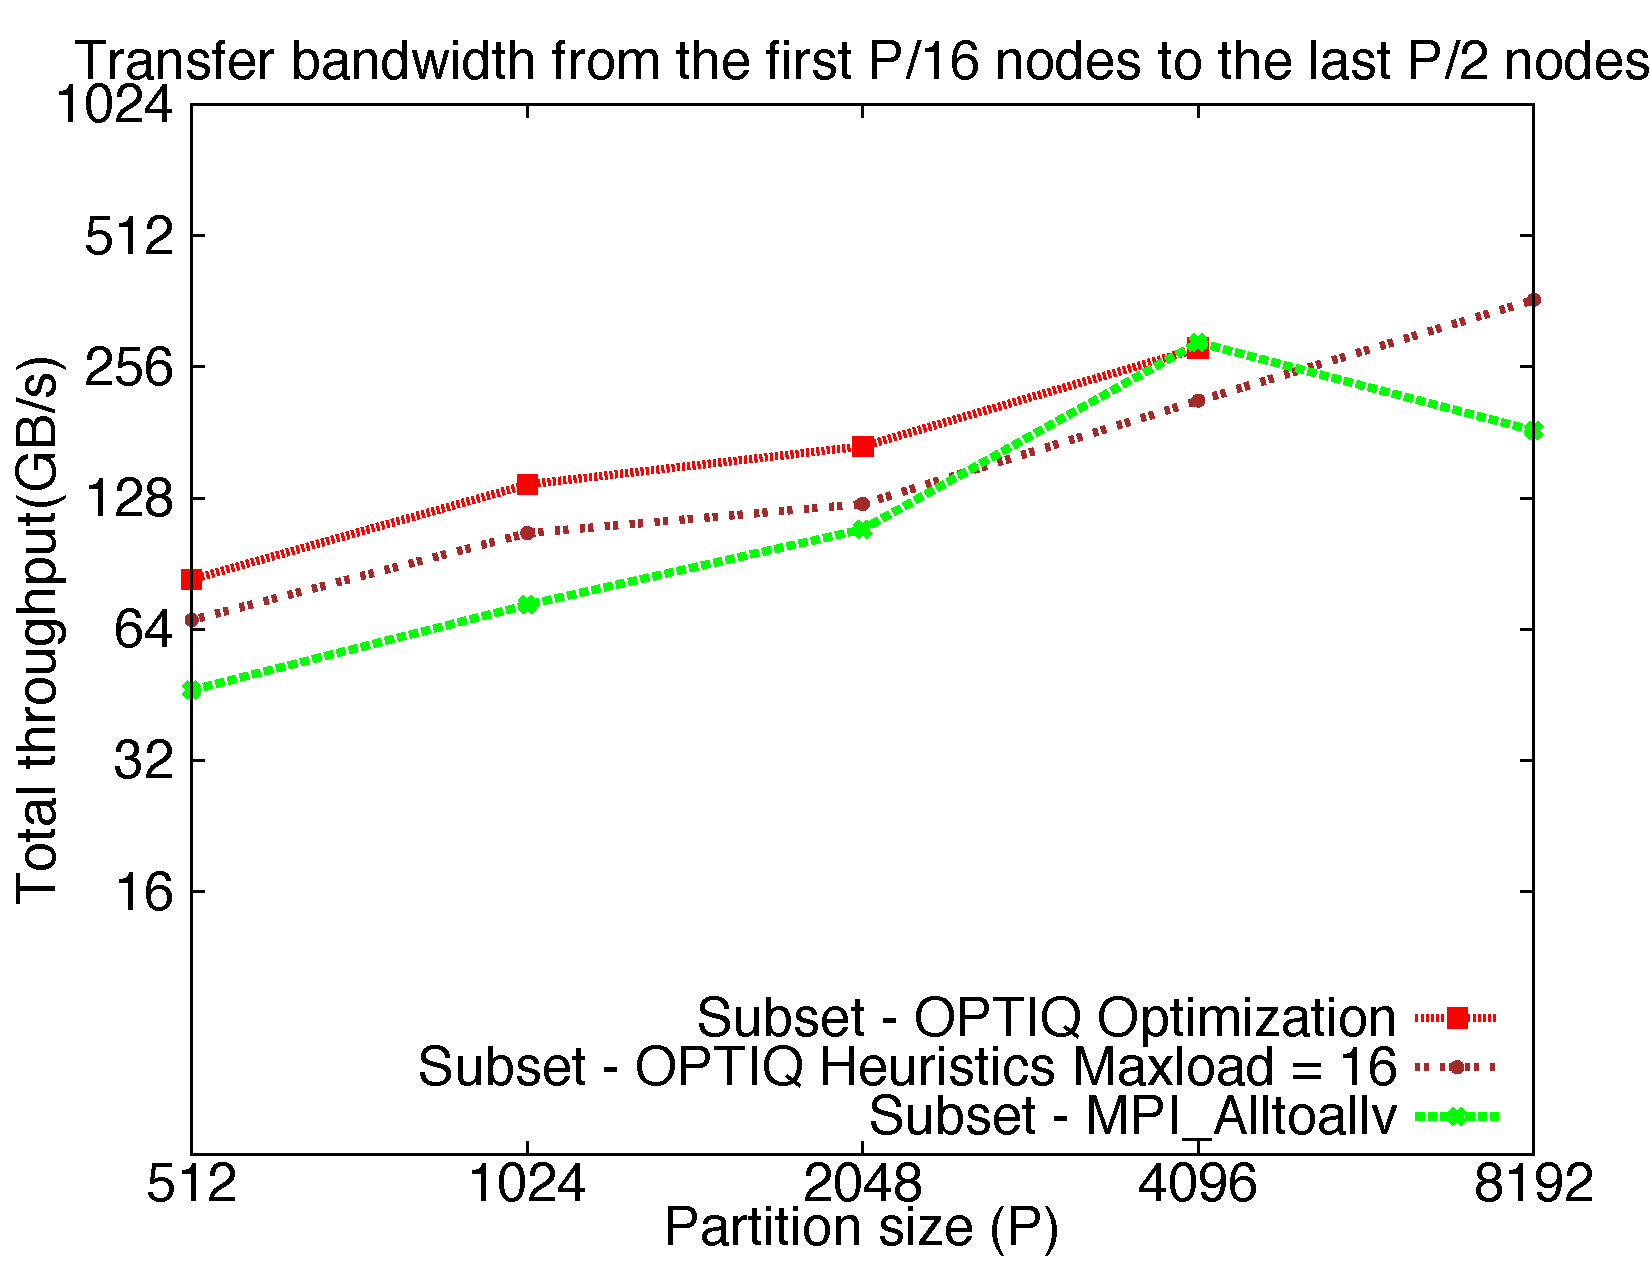
\includegraphics[width=\textwidth]{figures/constantr_87}
                \caption{Subset}
                \label{fig:constantr_87}
        \end{subfigure}
        \caption{Varying the number of sources and destinations and total number of nodes while keeping the ratio constant (1:8).}
        \label{fig:constantr}
\end{figure*}

\begin{table*}[!htbp]
   \centering
    \begin{tabular}{| l | l | r | r | p{0.5cm} | p{0.5cm} | p{0.5cm} | p{0.5cm} |p{0.5cm} | p{0.5cm} |p{0.5cm} | p{0.5cm} |p{0.5cm} | p{0.5cm} |}
    \hline
    \multirow{3}{*}{Pattern} & \multirow{3}{*}{Type} & \multirow{3}{1cm}{BW (GB/s)} & \multicolumn{3}{ c| }{Num. of Paths} & \multicolumn{2}{ c| }{Hopbytes} & \multicolumn{2}{ c| }{Num of copies}& \multicolumn{2}{ c| }{Num of paths} & \multicolumn{2}{ c| }{Total data} \\ \cline{4-6}
    & & & \multirow{2}{0.5cm}{Total Paths} & \multicolumn{2}{ c| }{Per Job} & \multicolumn{2}{ c| }{Per Path (MB)} & \multicolumn{2}{ c| }{Per Path}& \multicolumn{2}{ c| }{Per Link}& \multicolumn{2}{ c| }{Per Link (MB)} \\ \cline{5-14}
    & & & & {Max} & Avg & Max & Avg & Max & Avg & Max & Avg & Max & Avg\\ \hline
    \multirow{3}{*}{Disjont} & OPT    & 188.62 & 1,169 & 6 & 2.28 & 83.88 & 23.02 & 1152 & 295.22 & 11 & 2.53 & 18.28 & 9.26 \\ \cline{2-14}
    & HEU 16 & 74.88  & 3,146 & 23 & 6.14 & 83.88 & 8.45 & 1152 & 108.24 & 16 & 4.94 & 63.04 & 6.92 \\ \cline{2-14}
    & MPI    & 45.18  & 512  & 1 & 1.00 & 92.27 & 50.33 & & & 16 & 3.07 & 134.21 & 25.76\\ \hline
    \multirow{3}{*}{Overlap} & OPT    & 200.03 & 1303 & 6 & 2.54 & 83.88 & 19.28  & 1152 & 243.96 & 13 & 2.74 & 16.97 & 9.04\\ \cline{2-14}
    & HEU 16 & 113.17  & 3273 & 26 & 6.39 & 75.49 & 7.41 & 1024 & 93.07 & 16 & 5.17 & 38.66 & 7.04 \\ \cline{2-14}
    & MPI    & 42.84 & 512 & 1 & 1.00 & 83.88 & 42.99 &  & & 16 & 3.38 & 134.21 & 28.36 \\ \hline
    \multirow{3}{*}{Subset} & OPT    & 199.20 & 1269 & 6 & 2.48 & 75.49 & 19.48 & 1024 & 245.66 & 11 & 2.79 & 17.10 & 9.32 \\ \cline{2-14}
    & HEU 16 &  61.71 & 3238 & 26 & 6.32 & 75.49 & 7.43 & 1024 & 93.22 & 16 & 5.28 & 45.08  & 7.35 \\ \cline{2-14}
    & MPI    &  41.37 & 512  & 1 & 1.00 & 83.88 &  41.94 & & & 16 & 3.52 & 134.21 & 29.49 \\ \hline
    \end{tabular}
    \caption{Throughput, total num of paths, number of paths per job, maximum and average values of hopbytes, number of copies, number of paths per link and amount of data per link for 3 patterns in 1024 nodes experiments.}
    \label{table:constantr}
\end{table*}

In this experiment, we vary the number of sources, destinations together with total number of nodes while keeping the ratio between number of sources and destination 1/8. With the total number of nodes P  increases from 512 to 8192, the first P/16 nodes send data to the last P/2 nodes. Each source has 8 destinations e.g node 0 sends data to nodes P/2, P/2+1, ...P/2+7. We tested the framework for 3 patterns: subset, disjoint and overlap with 3 approaches of transferring data OPTIQ Optimization, OPTIQ Heuristics and MPI\_Alltoallv. We use 1 MPI/PAMI rank/node. The data size is 8 MB per pair. We set the max load equal 16 for the Heuristic approach.

As shown in Figure \ref{fig:constantr}, the Optimization approach has the highest throughput, the Heuristics approach is next and MPI\_Alltoall achieved the lowest throughput. The Table \ref{table:constantr} shows that in all 3 patterns the Heuristic with max load set to 16 was able to find highest number of paths. The Heurisc approach also has the highest maximum and average number paths for a job. As data is divided equally among paths, this led to lowest maximum and average values for hopbytes, number of copies per path. However, this led to higher number of paths per physical link higher amount of data per physical link of the Heuristic approach in comparison to the Optimization approach. In Optimization, the data is plit among paths to balance the amount of data between physical links, thus it has the lowest maximum amount of data per physical link. This led to its highest throughput. MPI\_Alltoall approach has the lowest number of paths. With 1 path per pair of communication, data is not split. Thus, it has the the highest hopbytes and data per physical link. Both factors led to its lowest throughput.


\subsubsection{Increasing sources-destinations distance}

In this experiment, we show that when distance between sources and destination increases, we are able to find more path while not increasing maximum load on physical links, thus improve performance. The experiment is done in 2048-node partition with the first 256 nodes (0-255) fixed as sources communicating with 512 destination nodes. The destination nodes location is moving to increase the number of hops between sources and destination from [256-767] to [512-1023], [768-1279] and [1024-1535].

\begin{figure*}[!htbp]
        \centering
        \begin{subfigure}[b]{0.32\textwidth}
                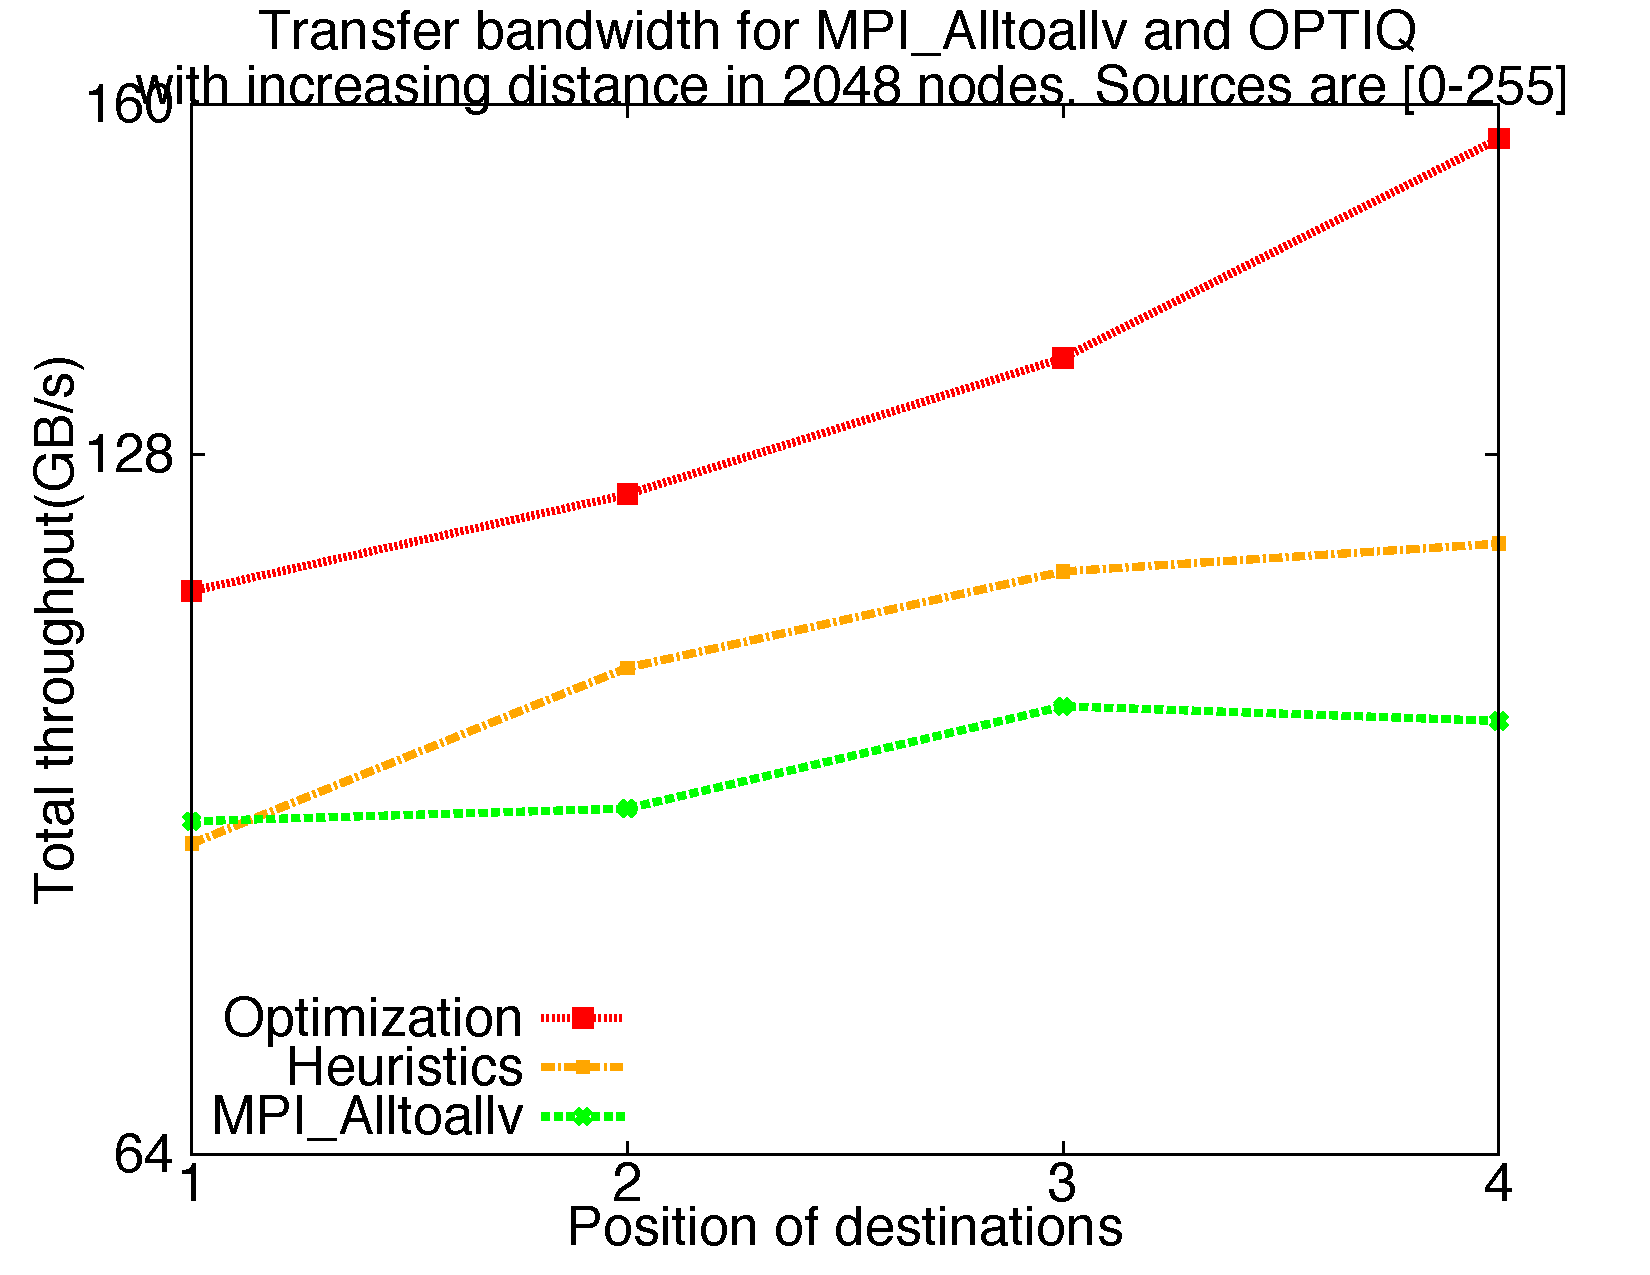
\includegraphics[width=\textwidth]{figures/incrdist_disjoint.pdf}
                \caption{Disjoint}
                \label{fig:incrdist_disjoint}
        \end{subfigure}%
        ~ %add desired spacing between images, e. g. ~, \quad, \qquad, \hfill etc.
          %(or a blank line to force the subfigure onto a new line)
        \begin{subfigure}[b]{0.32\textwidth}
                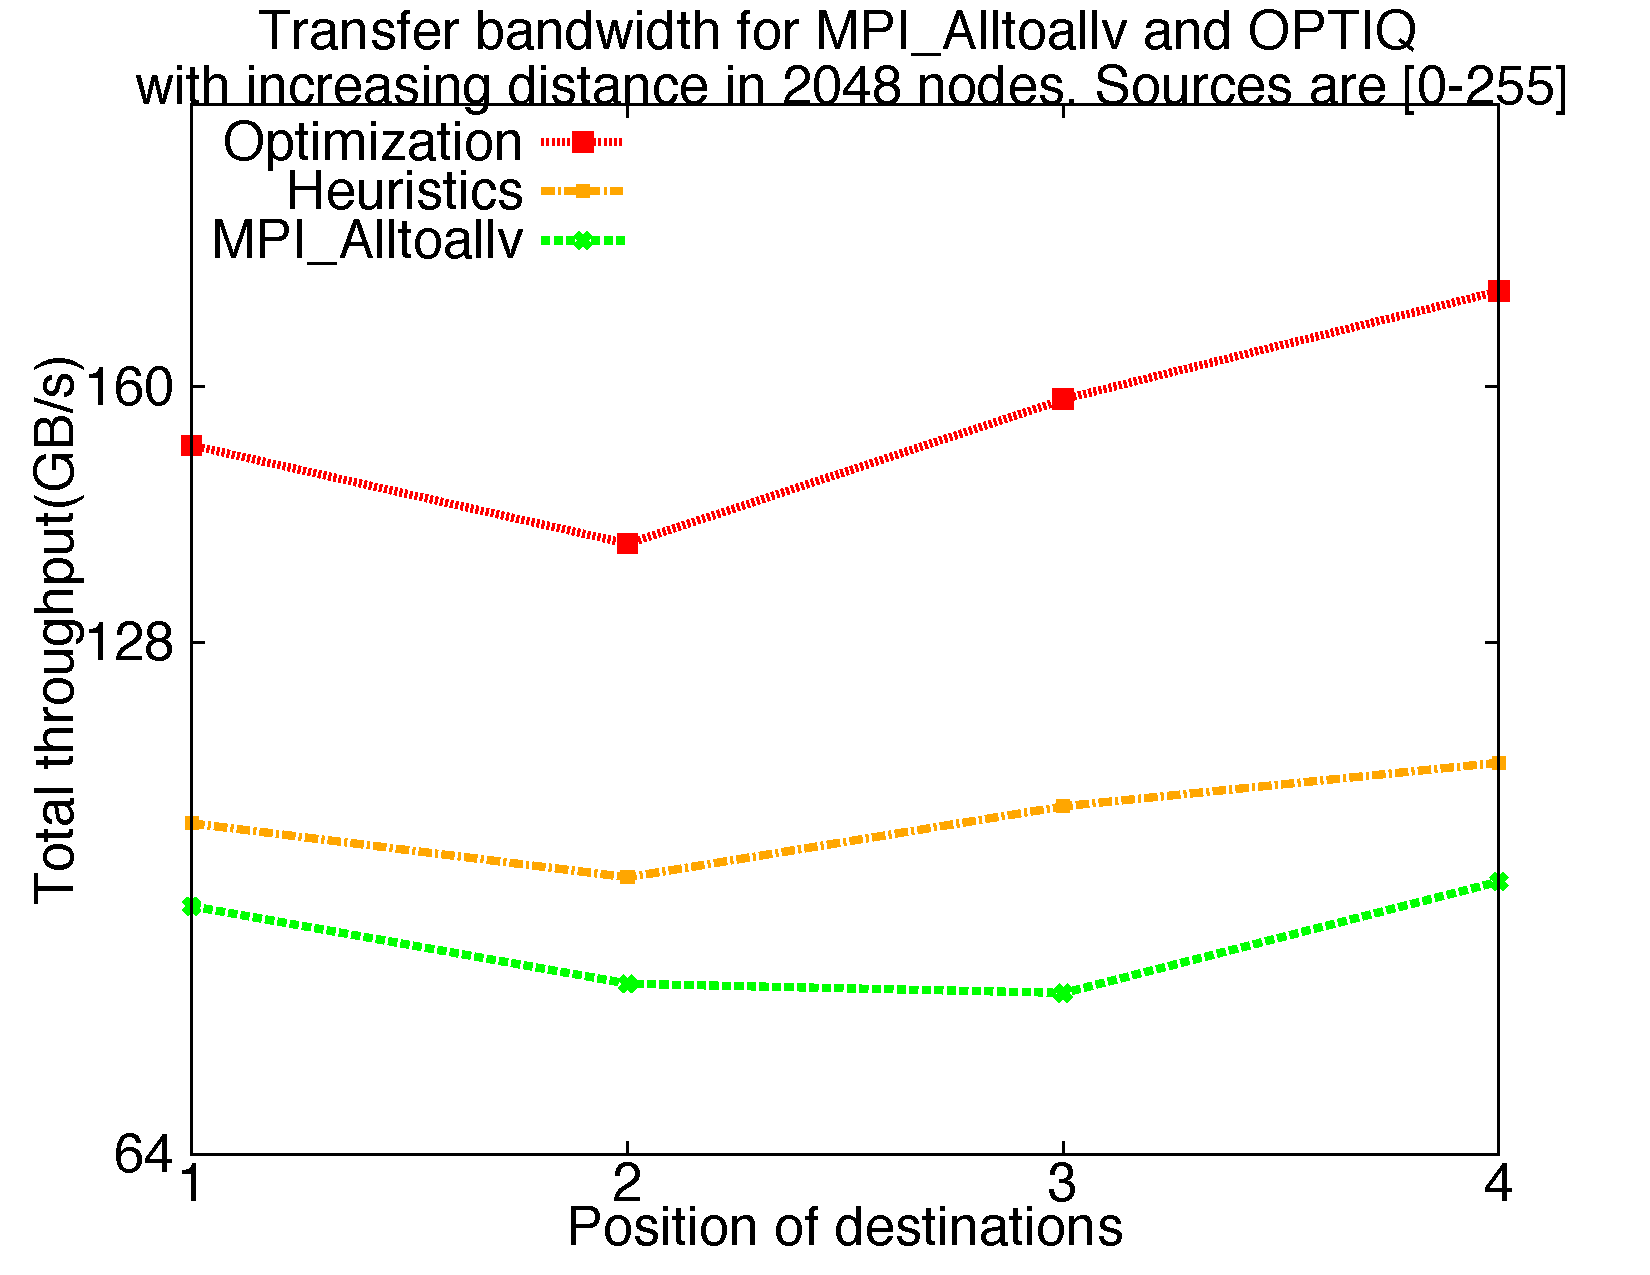
\includegraphics[width=\textwidth]{figures/incrdist_overlap}
                \caption{Overlap}
                \label{fig:incrdist_overlap}
        \end{subfigure}
        ~ %add desired spacing between images, e. g. ~, \quad, \qquad, \hfill etc.
          %(or a blank line to force the subfigure onto a new line)
        \begin{subfigure}[b]{0.32\textwidth}
                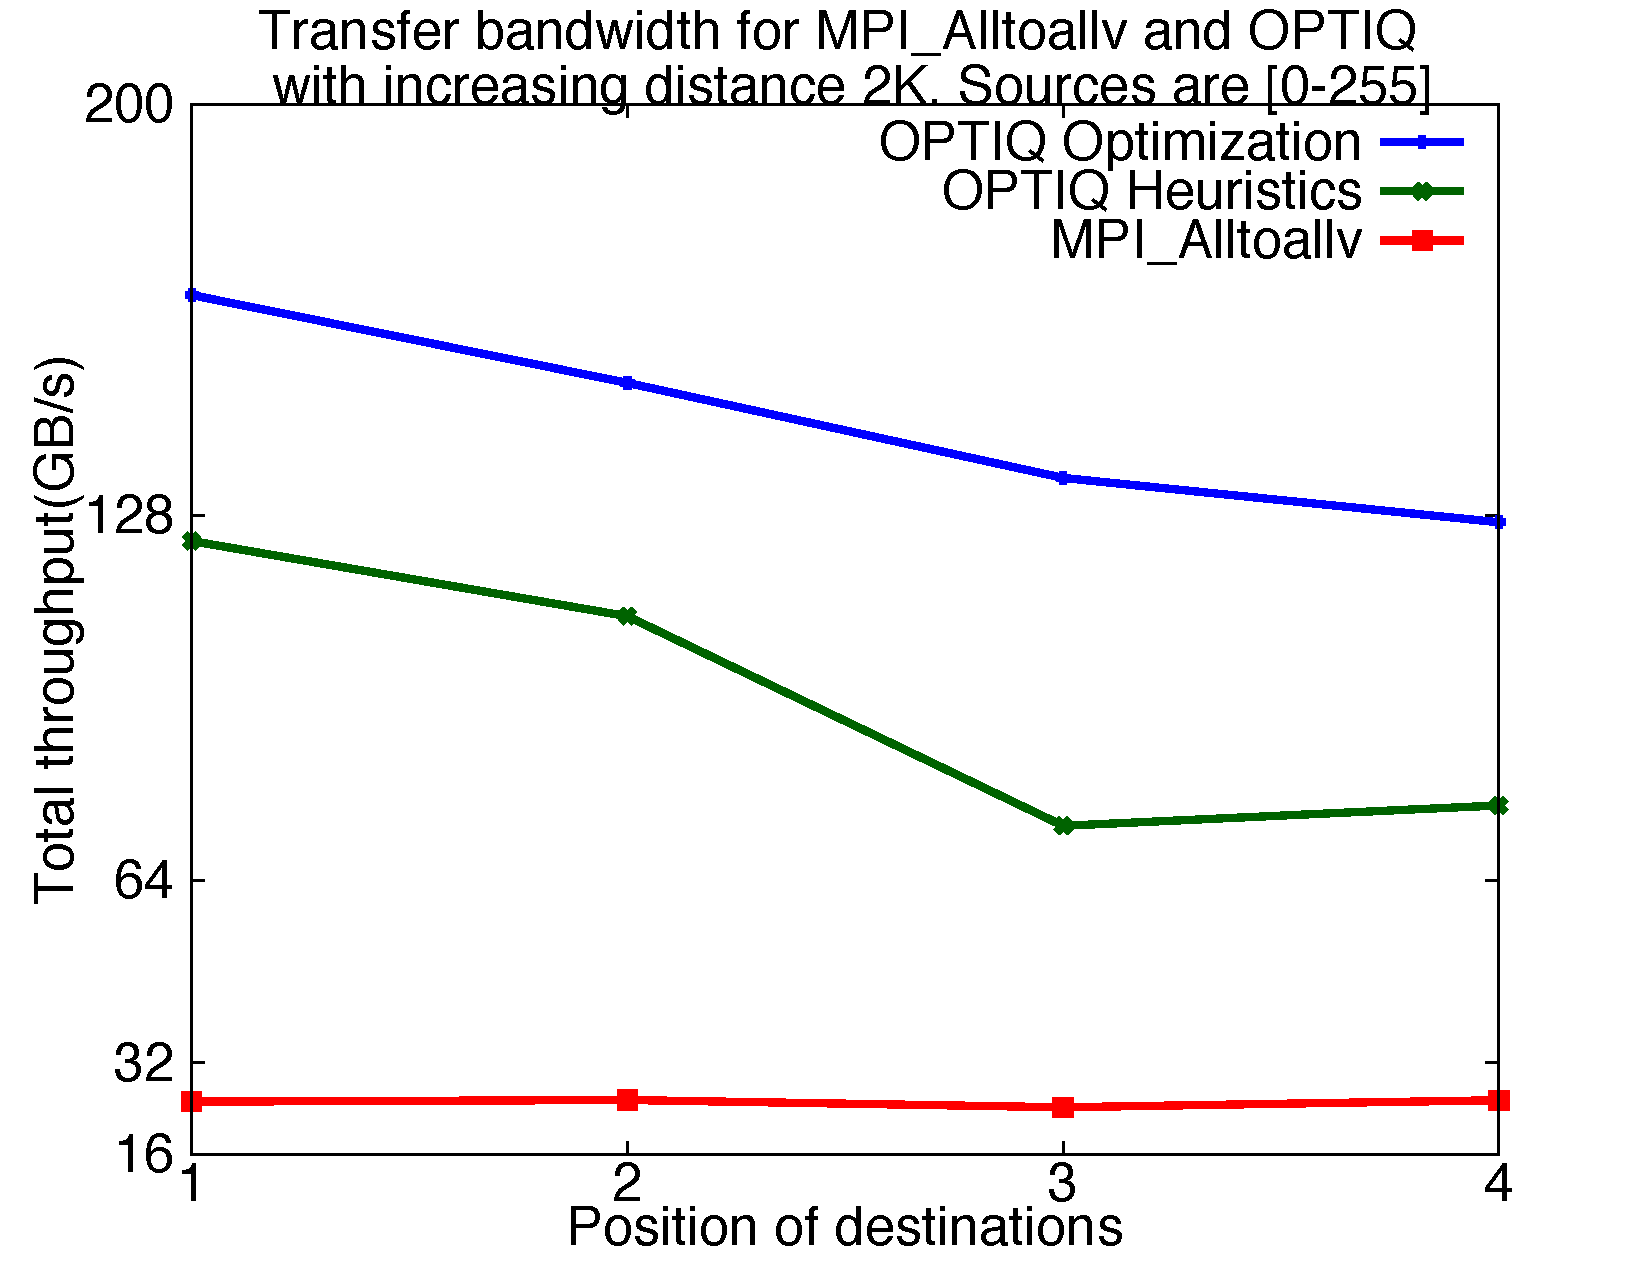
\includegraphics[width=\textwidth]{figures/incrdist_subset}
                \caption{Subset}
                \label{fig:incrdist_subset}
        \end{subfigure}
        \caption{Total data movement throughput when increasing distance between sources and destinations.}
        \label{fig:incrdist}
\end{figure*}

\begin{table*}[!htbp]
   \centering
    \begin{tabular}{| l | p{0.5cm} | p{0.5cm} | p{0.5cm} | p{0.5cm} | p{0.5cm} | p{0.5cm} |p{0.5cm} | p{0.5cm} | p{0.5cm} | p{0.5cm} |p{0.5cm} | p{0.5cm} |p{0.5cm} | p{0.5cm} |p{0.5cm} | p{0.5cm} |}
    \hline
     Positions & \multicolumn{4}{ c | }{1} & \multicolumn{4}{ c| }{2} & \multicolumn{4}{ c| }{3} & \multicolumn{4}{ c| }{4} \\ \hline
     Patterns & {Max} & Avg & Opt Paths & Heu Paths & Max & Avg & Opt Paths & Heu Paths & Max & Avg & Opt Paths & Heu Paths & Max & Avg & Opt Paths & Heu Paths \\ \hline
     Disjoint & 14 & 7.50 & 1105 & 2822 & 14  & 7.50 & 1372 & 2887 & 15 & 8.50 & 1547 & 3668 & 15 & 8.50 & 1672 & 3834 \\ \hline
     Overlap & 13 & 7.25 & 2085 & 6460 & 14  & 7.69 & 2152 & 3671 & 15 & 7.88 & 2337 & 6548 & 18 & 9.59 & 2399 & 7010 \\ \hline
     Subset &  20 & 8.56 & 1840 & 3422 & 21  & 8.56 & 1639 & 3364 & 22 & 9.06 & 1594 & 3119 & 23 & 9.06 & 1477 & 3087 \\ \hline
    \end{tabular}
    \caption{Maximum (Max) and average (Avg) distance (number of hops) and number of paths (Paths) between souces and destinations at each position.}
    \label{table:incrdist}
\end{table*}

The number of paths produced by Optimization approach are 1105 to 1372, 1547 and 1672 respectively. With increasing number of paths, the hopbytes, number of copies per paths and data load per physical link decrease, thus increasing in performance as shown in Figure \ref{fig:incrdist}. The same trend is observed in the Heuristics approach.


\subsubsection{Increasing number of destination nodes}
\label{sec:incrdestnodes}

\begin{figure*}%[!htbp]
        \centering
        \begin{subfigure}[b]{0.32\textwidth}
                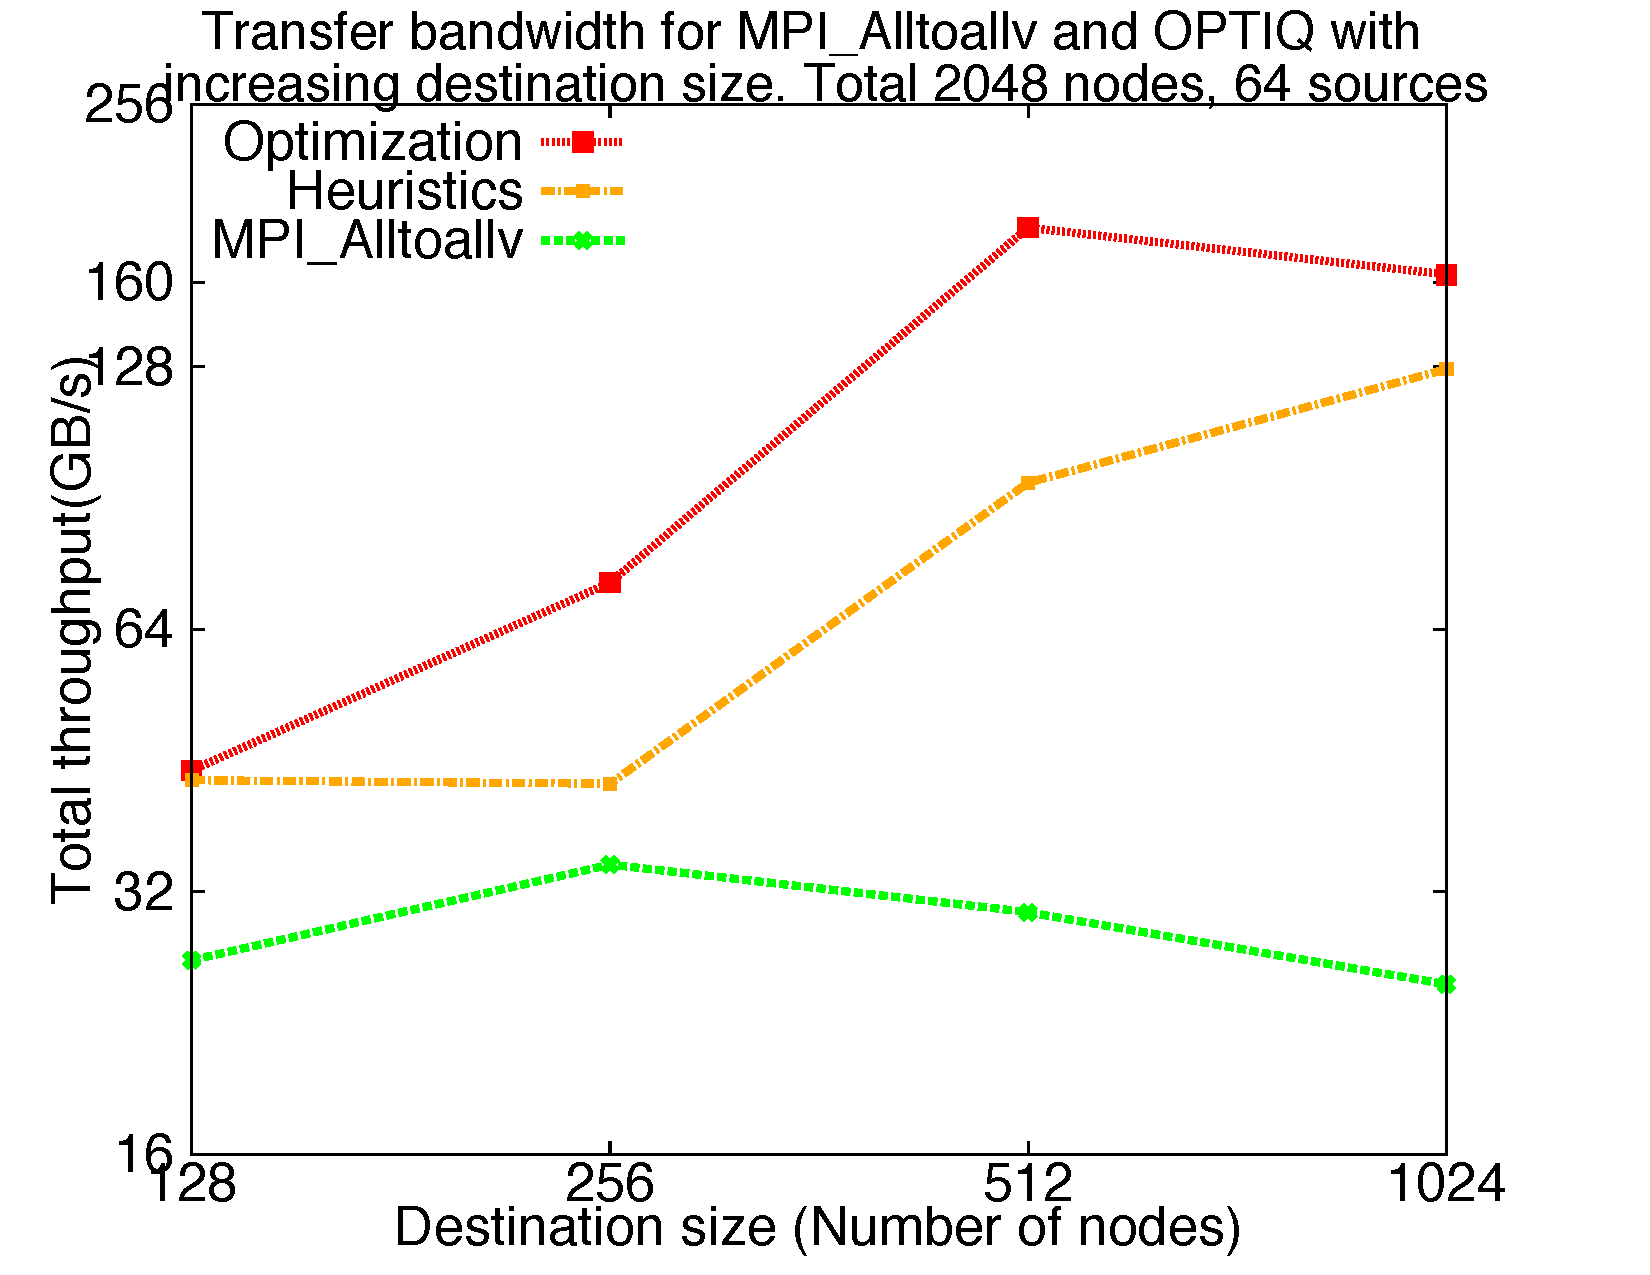
\includegraphics[width=\textwidth]{figures/incrsize_disjoint.pdf}
                \caption{Disjoint}
                \label{fig:incrsize_disjoint}
        \end{subfigure}%
        ~ %add desired spacing between images, e. g. ~, \quad, \qquad, \hfill etc.
          %(or a blank line to force the subfigure onto a new line)
        \begin{subfigure}[b]{0.32\textwidth}
                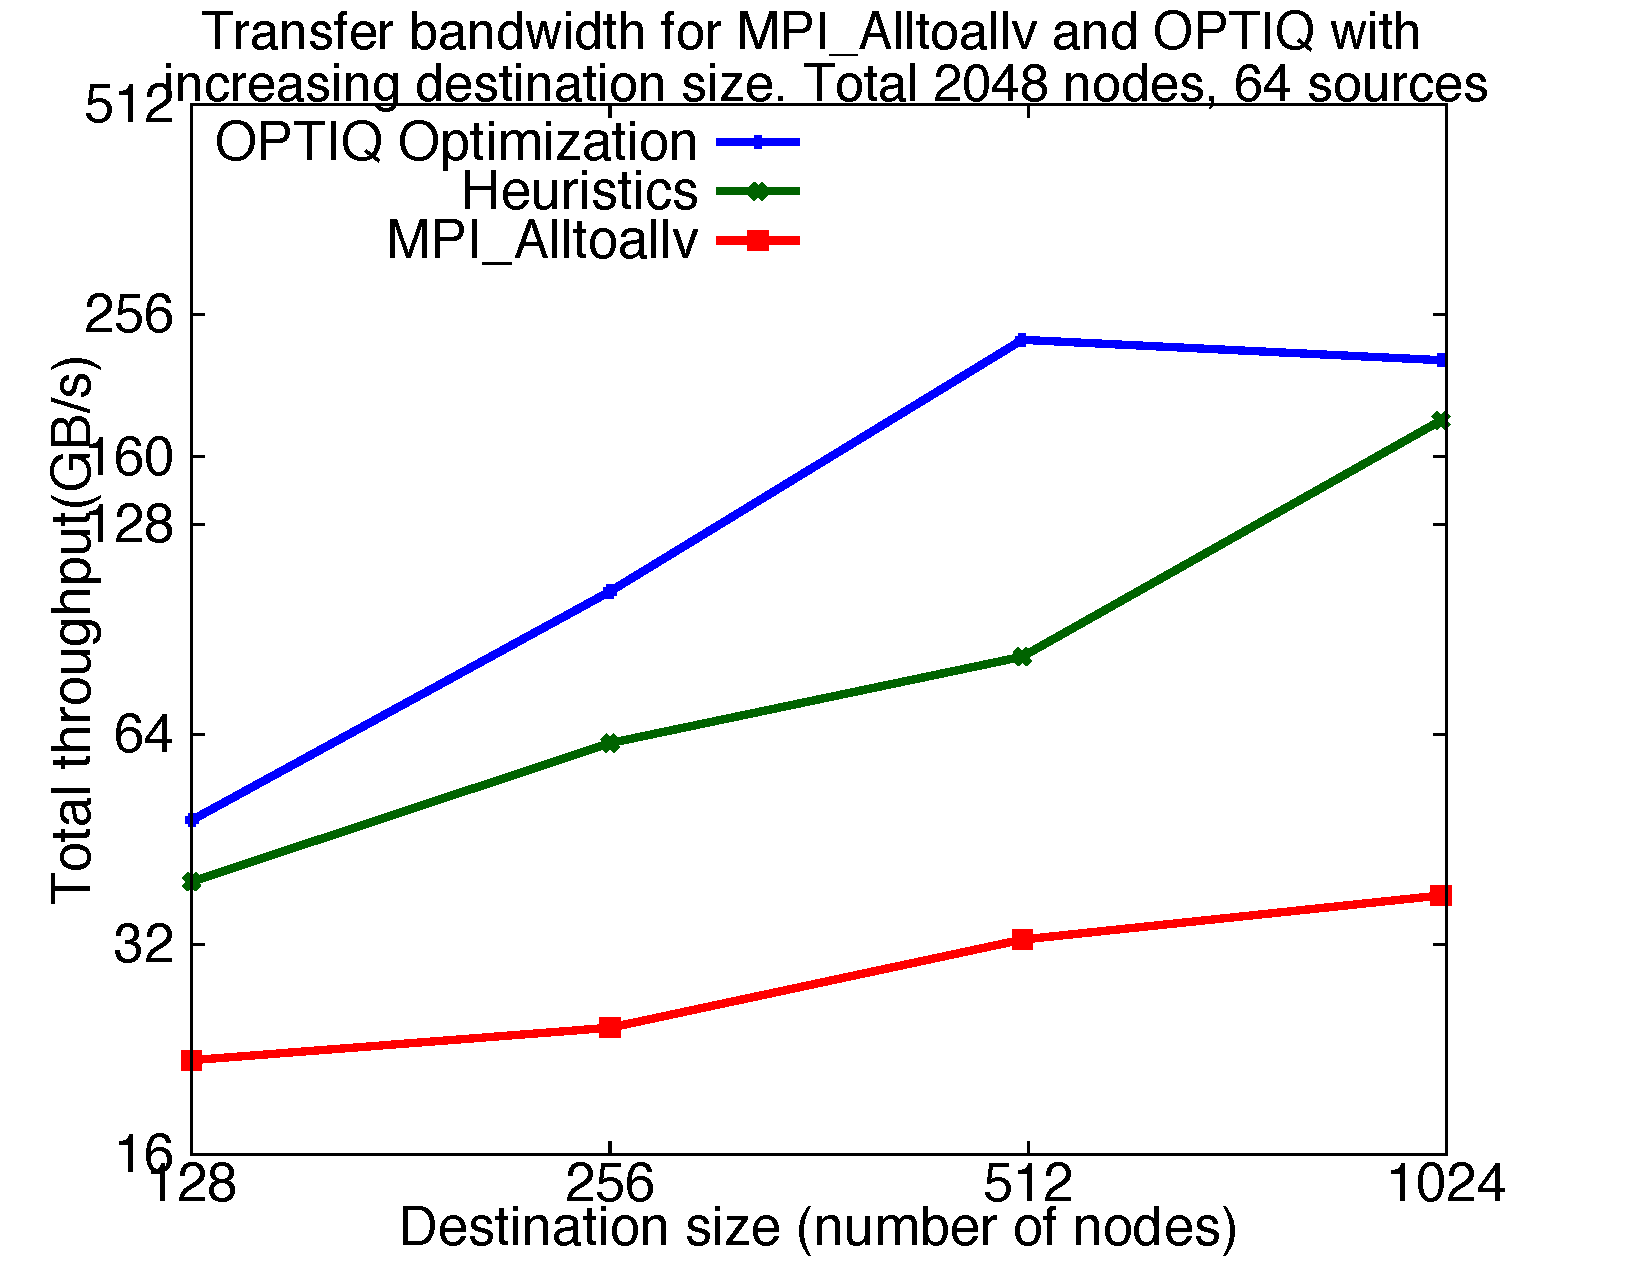
\includegraphics[width=\textwidth]{figures/incrsize_overlap}
                \caption{Overlap}
                \label{fig:incrsize_overlap}
        \end{subfigure}
        ~ %add desired spacing between images, e. g. ~, \quad, \qquad, \hfill etc.
          %(or a blank line to force the subfigure onto a new line)
        \begin{subfigure}[b]{0.32\textwidth}
                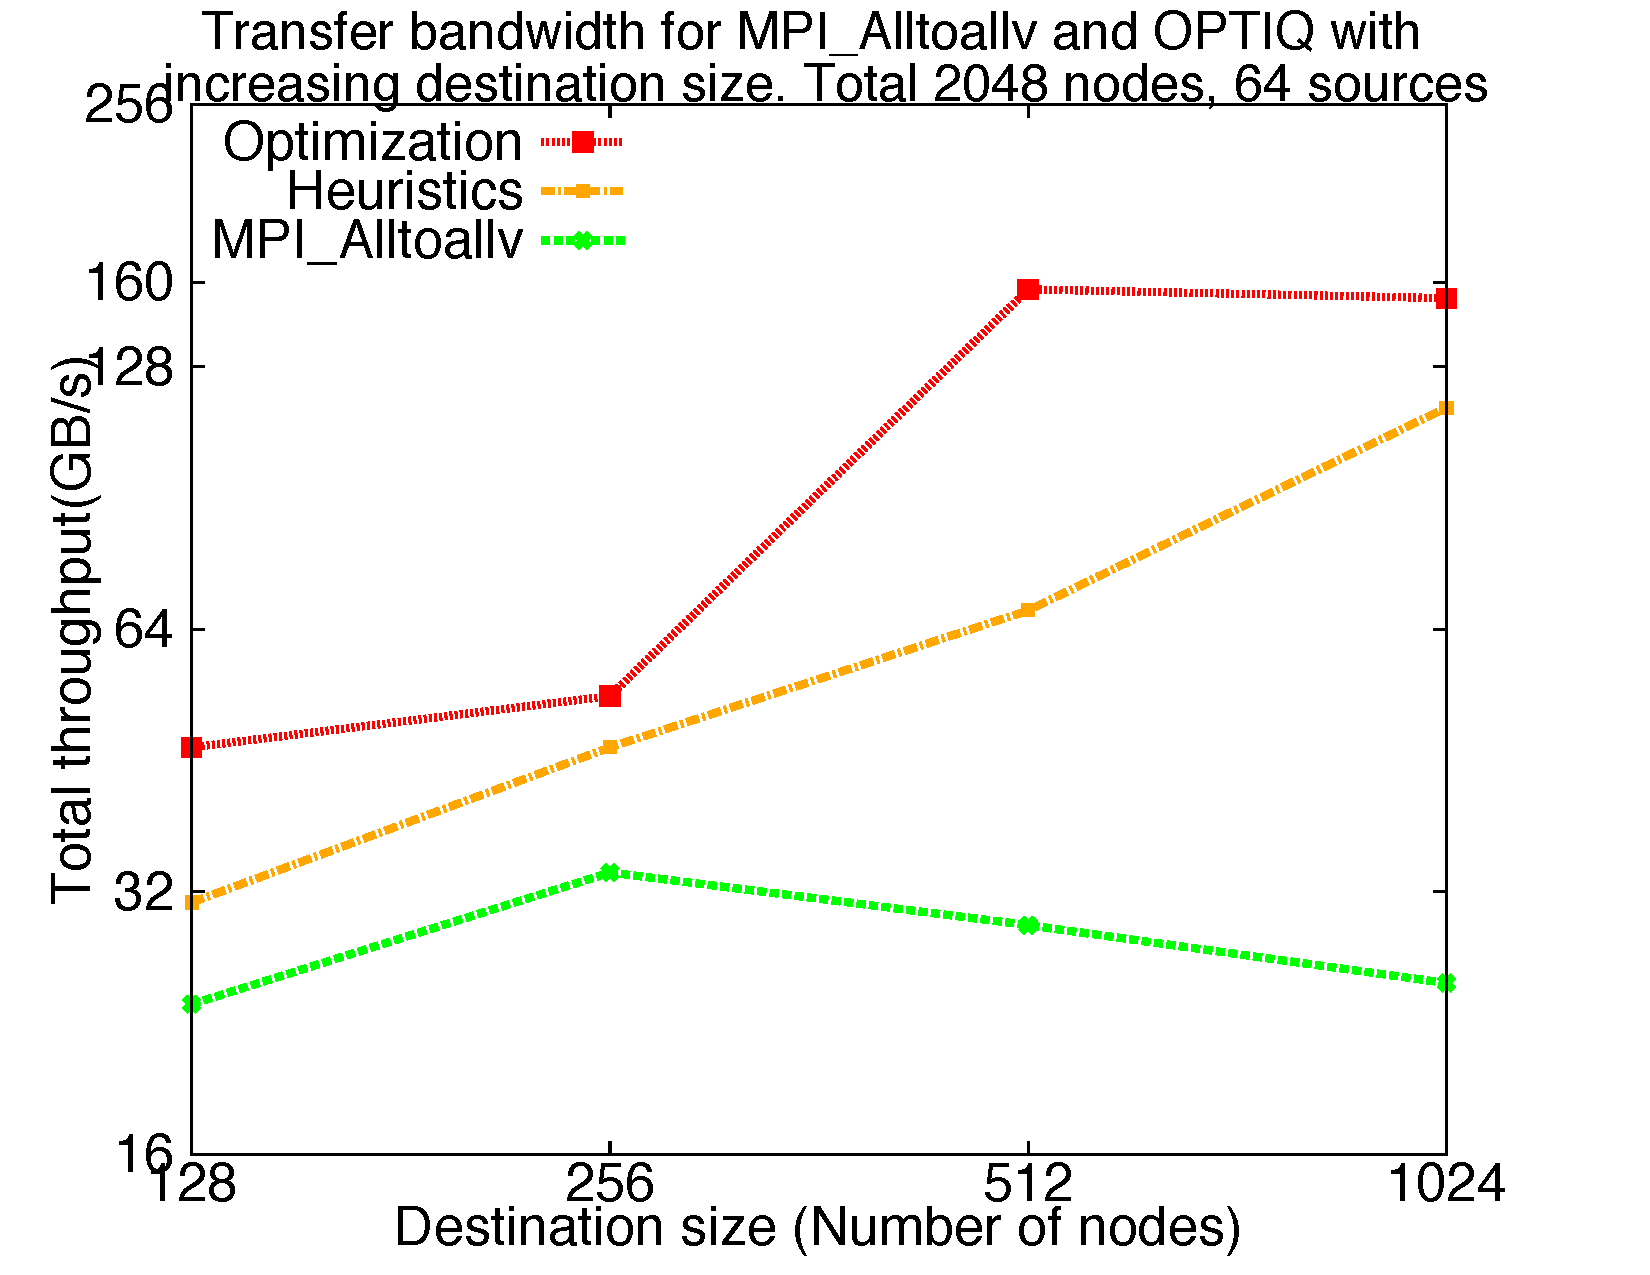
\includegraphics[width=\textwidth]{figures/incrsize_subset}
                \caption{Subset}
                \label{fig:incrsize_subset}
        \end{subfigure}
        \caption{Total data movement throughput when increasing destination size}
        \label{fig:incrsize}
\end{figure*}

In this experiment we use a partition of 2048 nodes. We keep the number of source nodes constant (64 nodes) and increase the number of destination nodes from 128 to 256, 512 and 1024 nodes. Each source node communicates with k destination nodes where k = 2, 4, 8 and 16 respectively. Node $x$ communicates with nodes $k\cdot x$, $k\cdot x+1$, ..., $k\cdot x+(k-1)$. There is 1 MPI/PAMI rank per node. Each pair of communication involves 8 MB of data transfer. The performance of OPT, HEU and MPI for disjoint, overlap and subset patterns is shown in Figure \ref{fig:incrsize}. With increase in number of destination nodes, OPT and HEU has better performance than MPI\_Alltoallv. The throughput of OPT increases for destination sizes of 256 and 512 but slightly reduces at 1024 nodes, whereas the throughput of HEU increases as the destination size increases. This is because OPT tries to globally balance load while distributing data among all paths, whereas HEU ensures load limit per path but distributes data for each communication pair, oblivious of the global load. Though OPT should yield better performance in all cases, we believe the reason for its drop in performance is that we do not consider the underlying synchronization overheads in the data transfer. 
%TODO why is this the case? higher load for OPT for 1024? review the above reason, does it seem correct?
%As Figure \ref{fig:incrsize} shows, as we increase the ratio between the sources and destinations by increasing the destination sizes, both Optimization and Heuristics have better performance than MPI\_Alltoallv. In addition, they work better at scale than MPI\_Alltoallv. The throughput of Optimization approach increases for destination sizes of 256 and 512 but slightly reduces at 1024 nodes, while the throughput of Heuristic approach increases as the destination size increases.
\begin{table*}%[!htbp]
   \centering
    \begin{tabular}{| l | p{0.5cm} | p{0.5cm} | p{0.6cm} | p{0.6cm} | p{0.5cm} | p{0.5cm} |p{0.6cm} | p{0.6cm} | p{0.5cm} | p{0.5cm} |p{0.6cm} | p{0.6cm} |p{0.5cm} | p{0.5cm} |p{0.6cm} | p{0.6cm} |}
    \hline
     \#destinations & \multicolumn{4}{ c | }{128} & \multicolumn{4}{ c| }{256} & \multicolumn{4}{ c| }{512} & \multicolumn{4}{ c| }{1024} \\ \hline
     Patterns & {Max} & Avg & OPT \#Paths & HEU \#Paths & Max & Avg & OPT \#Paths & HEU \#Paths & Max & Avg & OPT \#Paths & HEU \#Paths & Max & Avg & OPT \#Paths & HEU \#Paths \\ \hline
     Disjoint & 15 & 9.50 & 355 & 1021 & 18 & 10.44 & 923 & 1386 & 20 & 10.44 & 1101 & 1978 & 21 & 10.19 & 1631 & 1958 \\ \hline
     Overlap  & 11 & 6.25 & 476 & 2108 & 16 & 7.19 & 937 & 2864 & 18 & 8.38 & 1690 & 4064 & 21 & 9.12 & 2081 & 4710 \\ \hline
     Subset   & 11 & 5.5  & 491 & 1799 & 16 & 6.69 & 665 & 2184 & 20 & 8.31 & 1255 & 3021 & 21 & 8.56 & 1551 & 3436\\ \hline
    \end{tabular}
    \caption{Maximum (Max) and average (Avg) distance (number of hops) and number of paths (Paths) between souces and destinations at each position.}
    \label{table:incrsize}
\end{table*}


\subsubsection{Random pairing between sources and destinations}

In this experiment, we randomized the pairing between sources and destination to shuffle the well-aligned pairing that we have in the previous experiment. To demonstrate the sustained performance, we did experiment for all 3 patterns at 512 nodes, with 1 MPI/PAMI rank per node, 8 MB of data per communication. We used the same ratio 1/8 i.e 32 first nodes communicates with last 256 nodes. However, we randomized the pair of sources and destinations for 5 times to see the performance. The resuls are presented in Table \ref{table:randomperf}.

\begin{table*}[!htbp]
   \centering
    \begin{tabular}{| l | p{0.4cm} | p{0.4cm} | p{0.4cm} | p{0.4cm} | p{0.4cm} | p{0.4cm} | p{0.4cm} | p{0.4cm} | p{0.4cm} |p{0.4cm} | p{0.4cm} |p{0.4cm} | p{0.4cm} |p{0.4cm} | p{0.4cm} | p{0.4cm} | p{0.5cm} |p{0.4cm} |}
    \hline
     Positions & \multicolumn{3}{ c | }{Rand 1} & \multicolumn{3}{ c| }{Rand 2} & \multicolumn{3}{ c| }{Rand 3} & \multicolumn{3}{ c| }{Rand 4} & \multicolumn{3}{ c| }{Rand 5} & \multicolumn{3}{ c| }{Average}\\ \hline
     Patterns & MPI & OPT & HEU & MPI & OPT & HEU & MPI & OPT & HEU & MPI & OPT & HEU & MPI & OPT & HEU & MPI & OPT & HEU \\ \hline
     Disjoint & 63 &  91  & 83 &  85  & 106 & 66  & 73 &  97  & 69 &  78 &  92  & 80 &  75 &  105 & 73 & 74.8 & 98.2  & 74.2 \\ \hline
     Overlap  & 78 &  108 & 98 &  86  & 106 & 91  & 74 &  107 & 90 &  83 &  114 & 85 &  87 &  107 & 71 & 81.6 & 108.4 & 87.0\\ \hline
     Subset   & 44 &  90  & 76 &  41  & 83  & 85  & 46 &  93  & 86 &  40 &  95  & 81 &  40 &  85  & 74 & 42.2 & 89.2  & 80.4 \\ \hline
    \end{tabular}
    \caption{Throughtput (GB/s) for MPI\_Alltoallv (MPI), Optimization (OPT) and Heuristic (HEU) when randomizing pairing of sources and destination.}
    \label{table:randomperf}
\end{table*}

\begin{table}[!htbp]
   \centering
    \begin{tabular}{| l |p{0.80cm} | p{0.80cm} | p{0.80cm} | p{0.80cm} |p{0.80cm} |}
    \hline
     & Rand 1 & Rand 2 & Rand 3 & Rand 4 & Rand 5 \\ \hline
     Disjoint & 6.95 & 6.74 & 7.08 & 7.05 & 6.90 \\ \hline
     Overlap  & 5.05 & 5.06 & 5.07 & 5.08 & 5.08 \\ \hline
     Subset   & 5.04 & 4.95 & 5.10 & 4.90 & 5.12 \\ \hline
    \end{tabular}
    \caption{Average distance (number of hops) between sources and destinations in 5 randome cases.}
    \label{table:randomdist}
\end{table}

%\begin{table*}[!htbp]
%   \centering
%    \begin{tabular}{| l | p{0.4cm} | p{0.4cm} | p{0.4cm} | p{0.4cm} | p{0.4cm} | p{0.4cm} | p{0.4cm} | p{0.4cm} | p{0.4cm} |p{0.4cm} | p{0.4cm} |p{0.4cm} | p{0.4cm} |p{0.4cm} | p{0.4cm} | p{0.4cm} | p{0.5cm} |p{0.4cm} |}
%    \hline
%     Positions & \multicolumn{3}{ c | }{Rand 1} & \multicolumn{3}{ c| }{Rand 2} & \multicolumn{3}{ c| }{Rand 3} & \multicolumn{3}{ c| }{Rand 4} & \multicolumn{3}{ c| }{Rand 5} \\ \hline
%     Patterns & Total & Max & Avg  & Total & Max & Avg  & Total & Max & Avg & Total & Max & Avg & Total & Max & Avg \\ \hline
%     Disjoint & 1779 & 12 & 6.95 & 1726 & 12 & 6.74 & 1806 & 11 & 7.08 & 1790 & 12 & 7.05 & 1753 & 12 & 6.90 \\ \hline
%     Overlap  & 1288 & 10 & 5.05 & 1291 & 10 & 5.06 & 1292 & 10 & 5.07 & 1295 & 10 & 5.08 & 1279 & 9 & 5.08 \\ \hline
%     Subset   & 1289 & 10 & 5.04 & 1267 & 10 & 4.95 & 1306 & 11 & 5.10 & 1254 & 10 & 4.90 & 1310 & 10 & 5.12 \\ \hline
%    \end{tabular}
%    \caption{Distance between sources and destinations: Total, Maximum and Average number of hops in 5 randome cases}
%    \label{table:randomdist}
%\end{table*}

As we see in the Table \ref{table:randomperf}, the performance of MPI\_Alltoallv and Optimization approach both varies when randomizing pairs of sources and destination. However, the Optimization is significantly higher thatn MPI\_Alltoallv. This is because Optimization was able to find more paths to transfer data (530-630 paths) than MPI\_Alltoallv (256 paths). The Optimization approach also had lower average and median values of hopbytes and amount of data per physical link. The experiment shows that even we randomize pairing of sources and destination, we still are able to achieve better performance.


\subsubsection{Benchmark for chunk size}

To transfer dat through intermediate, we split a message into smaller chunks and keep sending the chunks into the network. It is to reduce the waiting time at the intermediate, thus, reduce the total transfer time. We carried out an experiment to show optimal chunk sizes for different message sizes. In this experiment, we varied the message sizes from 8 KB up to 8 MB. The chunk sizes also varied from 4KB up to 1MB. The experiment is done in 512-node partition using subset pattern in which first 32 nodes send data to last 256 nodes. The results are shown in Figure \ref{fig:chunksize}.

\begin{figure}[!htb]
\vspace{-0.1in}
\centering
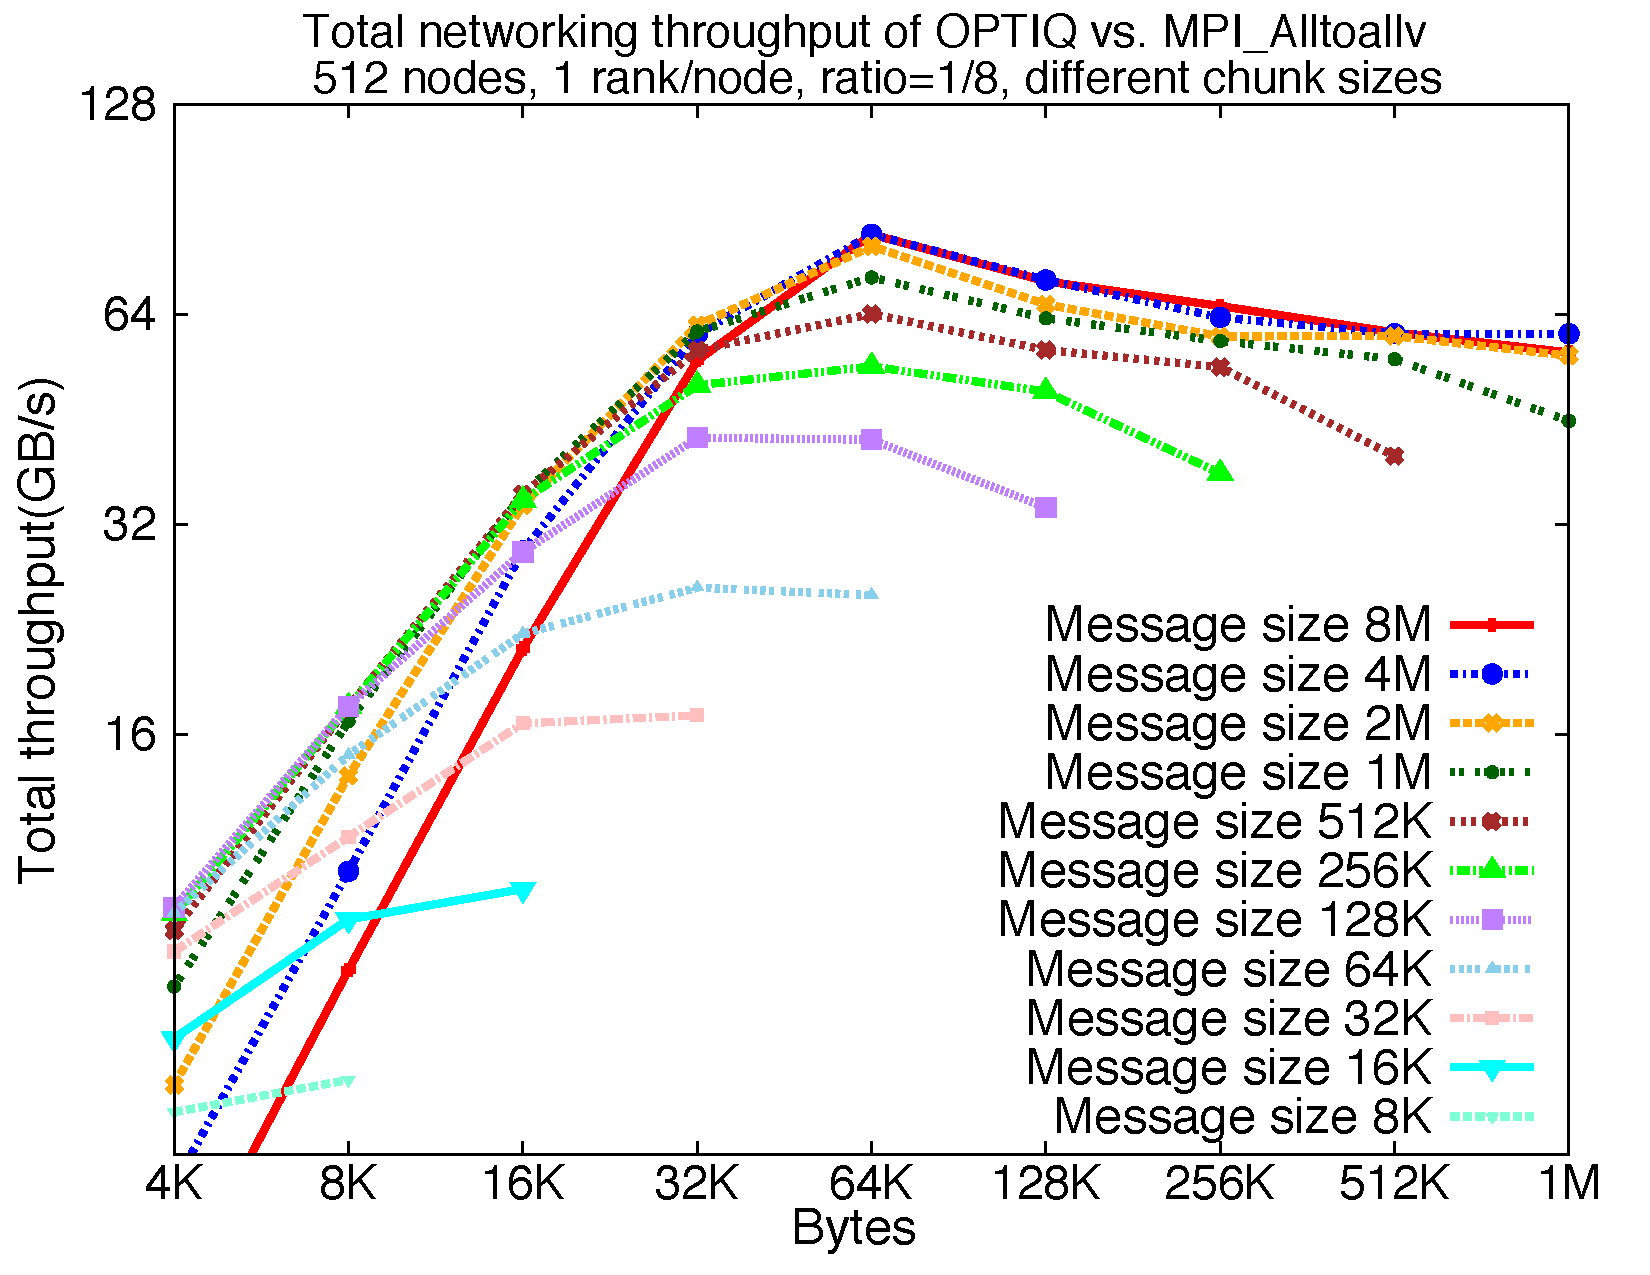
\includegraphics[scale=0.30]{figures/87_chunksize.pdf}
\vspace{-0.1in}
\caption{Chunk sizes and their performance in 512-node partition, subset pattern.}
\vspace{-0.1in}
\label{fig:chunksize}
\end{figure}

As shown in the Figure \ref{fig:chunksize}, for messages with sizes less than 16 KB, we should transfer the entire mesasges. With message size 32 KB, we can use chunksize 16 KB. With message sizes 64 KB or 128 KB, we can use 32 KB chunksize. With larger message sizes, we can use 64 KB chunk size. Similar trends are found in disjoint and overlap patterns. For the expriments in this paper, we use 64 KB chunk size.



\subsubsection{Performance in different message sizes}

Due to overheads in data transfer by OPTIQ, throughput of tranferring small messages might be degraded and lower than default MPI\_Alltoallv. In this experiment, we show effective message sizes for OPTIQ. The expriment is carried out in 512-node partition with 1 MPI/PAMI rank per node, 8 MB message size for all 3 patterns. The results are shown in Figure \ref{fig:messagesize}.

\begin{figure}[!htb]
\vspace{-0.1in}
\centering
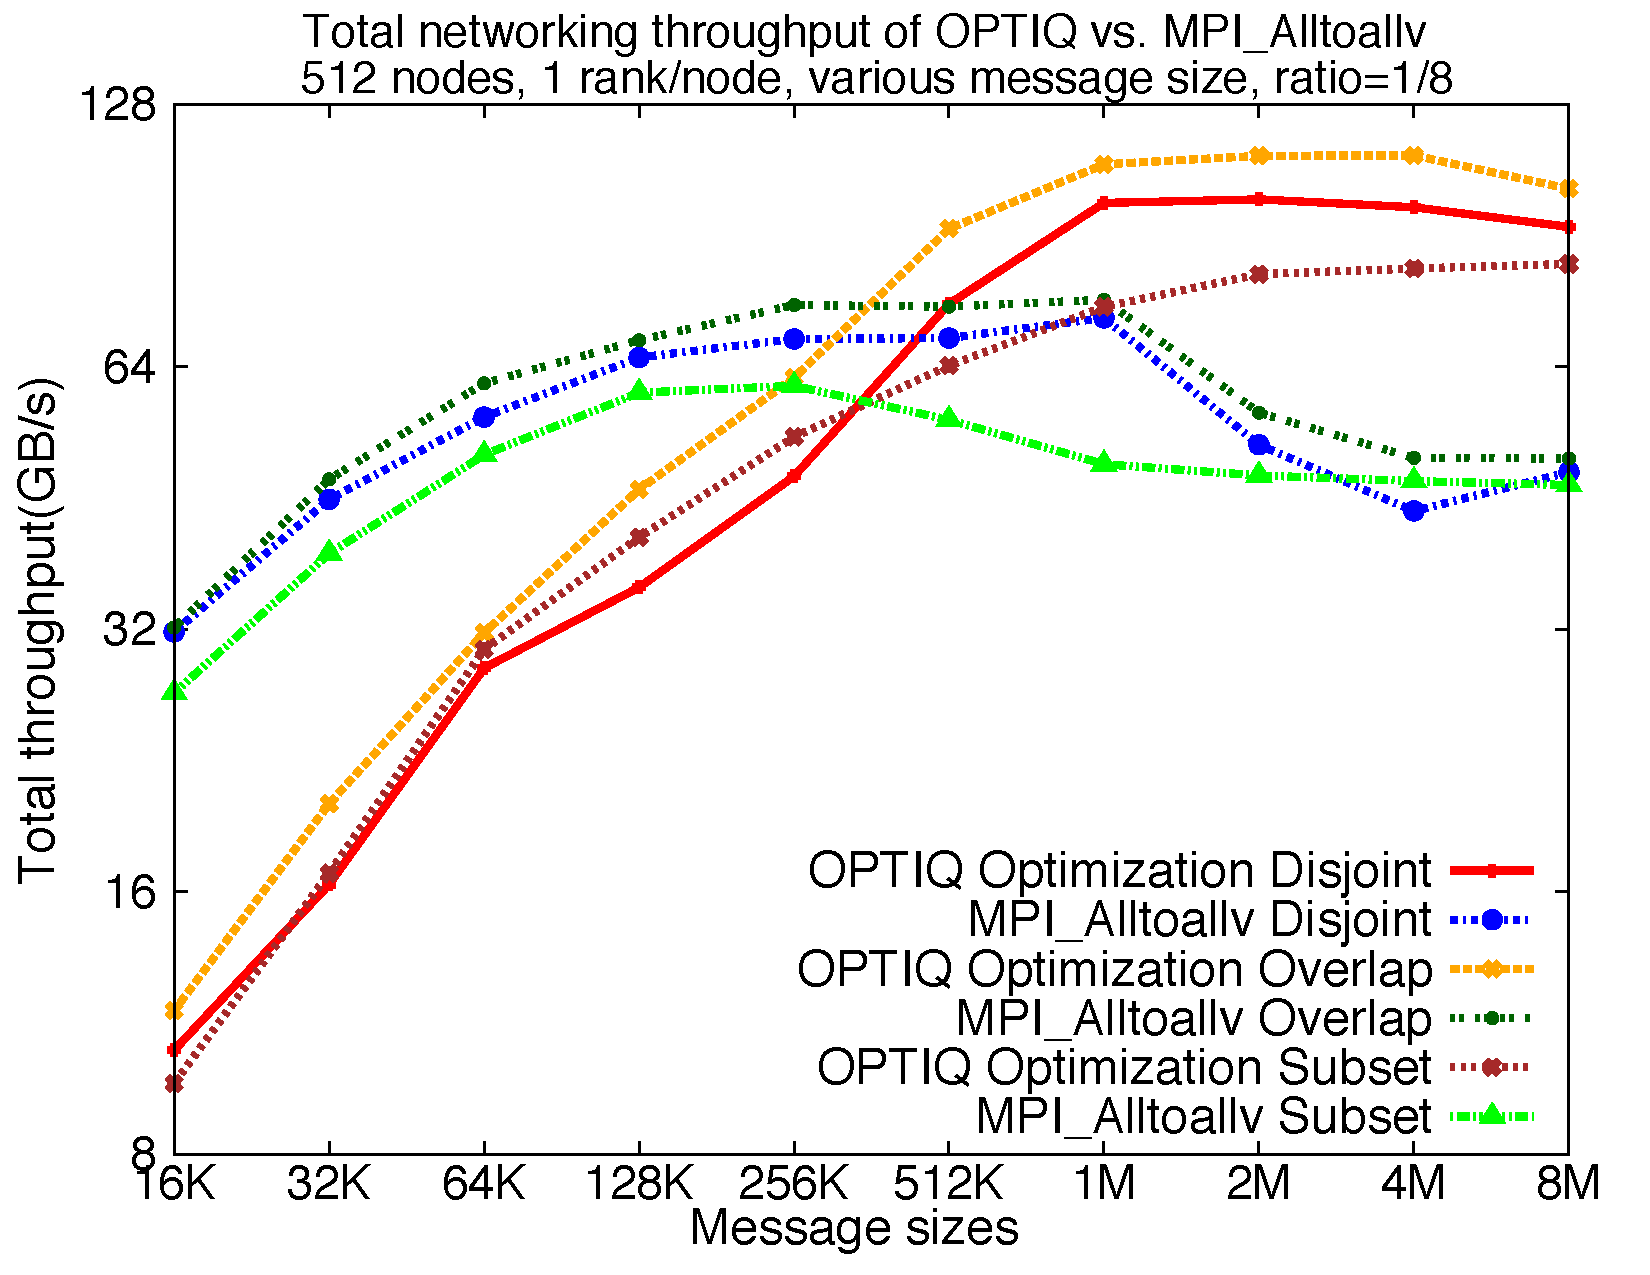
\includegraphics[scale=0.30]{figures/messagesize.pdf}
\vspace{-0.1in}
\caption{Total throughtput with different message sizes in 3 patterns.}
\vspace{-0.1in}
\label{fig:messagesize}
\end{figure}

As shown in the Figure \ref{fig:messagesize}, data transfer throughput flips at the size in between 256 KB and 512 KB. If the message size is less than 256 KB, MPI\_Alltoallv has better performance. When the message size is over 512 KB, OPTIQ has better performance. This is due to overheads caused by extra headers in each message, the time to copy and inject at each intermediate nodes.



\subsubsection{Maxload value for heuristic approach}

For the heuristic approach, we need to feed k shortest paths and a \textit{maxload} value to select a number of path used for data transfer. Depending on the number of \textit{maxload} value, we have different set of paths which can affect to the performance.  In this experiment, we show effectiveness of choosing the \textit{maxload} value and time to select paths based on the \textit{maxload} value. The expriment is carried out in 1024-node partition, with 1 MPI/PAMI rank per node, 8 MB message size, ratio 1/8 for all 3 patterns. The \textit{maxload} value varied from 1, 2, 4, 8, 16 to 32. The results are shown in Table \ref{table:maxload}.

\begin{table}[!htbp]
   \centering
    \begin{tabular}{| l |p{0.5cm} | p{0.5cm} |  p{0.5cm} | p{0.5cm} | p{0.5cm} | p{0.5cm} | p{0.75cm} |}
    \hline
     \multirow{2}{*}{Patterns} & \multirow{2}{*}{MPI} & \multicolumn{6}{ c| }{Number of paths} \\ \cline{3-8}
     & & 1 & 2 & 4 & 8 & 16 & 32 \\ \hline
     Disjoint & 45 & 31 & 32 & 32 & 63 & 75 & 78 \\ \hline
     Overlap & 42 & 66 & 66 & 66 & 125 & 112 & 89 \\ \hline
     Subset & 74 & 69 & 70 & 69 & 114 & 110 & 96 \\ \hline
    \end{tabular}
    \caption{Throughput (GB/s) with different \textit{maxload} values for Heuristic approach.}
    \label{table:maxload}
\end{table}

As shown in the Table \ref{table:maxload}, when the \textit{maxload} value is set to 1, 2 or 4, the performance is very much similar. They have the performance lower than MPI\_Alltoallv in Disjoint and Subset pattern. We gain the best performance with \textit{maxload} value set to 8 or 16. When the \textit{maxload} value is set to 32, the performance start to degrade in case of Overlap and Subset patterns while only increasing slightly in Disjoint pattern. This is because when the \textit{maxload} value is set to low values (1,2,4), the heuristic algorithm is not able to find enought paths to transfer data leading to fewer number of physical links being used, thus higher load on physical links. When the \textit{maxload} value set to high value (32), the heuristic algorihtm find too many paths leading to many paths sharing a physical link, thus higher load on physical links too. The performance is optimal with the \textit{maxload} value set to 8 or 16. With the values, we have appropriate number of links and the load is ditributed better on the physical links. For expriments in this paper, we set \textit{maxload} value to 16.

When we increase the \textit{maxload} value, it also takes more time to select paths from k shortest paths. The Table \ref{table:solvetime} shows the time for differnt \textit{maxload} values in deffernt patterns.

\begin{table}[!htbp]
   \centering
   \begin{tabular}{| p {0.75cm}| r | r | r | r | r | r |}
    \hline
    \multirow{2}{*}{Pattern} & \multicolumn{6}{ c| }{Time for Different Max Load (s)} \\ \cline{2-7}
    & 1 & 2 & 4 & 8 & 16 & 32 \\ \hline
    Disjoint & 1.958 & 1.961 & 1.917 & 1.956 & 2.002 &  2.164 \\ \hline
    Overlap & 1.923 & 1.890 & 1.801 & 1.929 & 1.993 & 2.082 \\ \hline
    Subset & 1.907 & 1.870 & 1.891 & 1.955 & 2.024 &  2.223 \\ \hline
    \end{tabular}
    \caption{Search time with diffent max load in 1024 nodes partition.}
    \label{table:solvetime}
\end{table}

The search time is short and thus, can be amortized over time when a pattern is used repeatedly.


\subsubsection{Number of paths fed into model}

For the Optimization approach we need to feed k shortest paths into solvers to search for an assigment of flow values for the k paths. In this experiment we show the relationship between the number of paths fed into the solvers and the corresponding data transfer throughput and the elapsed time for AMPL model and solvers. We carried out the experiment in a 2048-node partition for all three patterns at the ratio of 1:8 where 128 nodes communicates with 1024 nodes with the same pairing as the previous cases. We used 1 MPI/PAMI rank per node and 8 MB per communication.  We varied the number of paths fed into the solvers from 4 to 16, 32 and 50. The performance is shown in Table \ref{table:pathsintomodel}.

\begin{table}[!htbp]
   \centering
    \begin{tabular}{| l | p{0.5cm} | p{0.5cm} | p{0.5cm} | p{0.5cm} | p{0.75cm} |}
    \hline
     \multirow{2}{*}{Patterns} & \multirow{2}{*}{MPI} & \multicolumn{4}{ c| }{Number of paths} \\ \cline{3-6}
     & & 4 & 16 & 32 & 50 \\ \hline
     Disjoint & 61 & 29 & 84 & 104 & 197 \\ \hline
     Overlap & 59 & 82 & 192 & 224 & 308 \\ \hline
     Subset & 111 & 99 & 163 & 168 & 172 \\ \hline
    \end{tabular}
    \caption{Throughput (GB/s) with different number of paths fed into solvers.}
    \vspace{-0.15in}
    \label{table:pathsintomodel}
\end{table}

As shown in the Figure \ref{table:pathsintomodel}, as we increase the number of paths fed into the solvers, the performance increases. This is because with more paths the solvers have a larger search space, and thus can produced more optimal results to be used for data transfer. However, when increasing the number of paths, we also increase the time for AMPL model to prepare and sovlers to search for flow values for paths. The time spent by AMPL model and sovlers are shown in Table \ref{table:solvetime}.

\begin{table}[!htbp]
   \centering
   \begin{tabular}{| p {0.75cm}| p{0.5cm} | r | p{0.5cm} | p{0.5cm} | r | r | r | r |}
    \hline
    \multirow{2}{*}{Pattern} & \multicolumn{4}{ c| }{AMPL time (s)} & \multicolumn{4}{ c| }{Solve time (s)} \\ \cline{2-9}
    & 4 & 16 & 32 & 50 & 4 & 16 & 32 & 50 \\ \hline
    Disjoint & 13.9 & 187.7 & 123.0 & 224.0 & 0.06 & 6.6 & 4.4 & 84.0 \\ \hline
    Overlap & 13.6 & 51.9 & 134.6 & 198.7 & 0.09 & 16.6 & 179.4 & 530.3 \\ \hline
    Subset & 14.4 & 50.6 & 134.9 & 217.3 & 0.85 & 111.3 & 173.2 & 939.6 \\ \hline
    \end{tabular}
    \caption{AMPL and solving time.}
    \vspace{-0.15in}
    \label{table:solvetime}
\end{table}


\begin{comment}
\subsubsection{Subset - Type 2 (Subgroup Data Aggregation)}

In the subgroup data aggregation experiment, we aggregated data within a subgroup to one node in the subgroup. In this experiment, we used a 512-nodes partition. The partition was divided into subgroup of size 4, 8, 16, 32, and 64 nodes each. One node in the middle of a subgroup was selected as the destination to aggregate data from all nodes in the subgroup(including itself). The data size is 1MB. We aggregate data using MPI\_Alltoallv and our framework for 20 times, measured and reported the average of the measurements. The aggregation bandwidths are shown in Figure \ref{fig:aggbw}.

\begin{figure}[!htb]
\vspace{-0.1in}
\centering
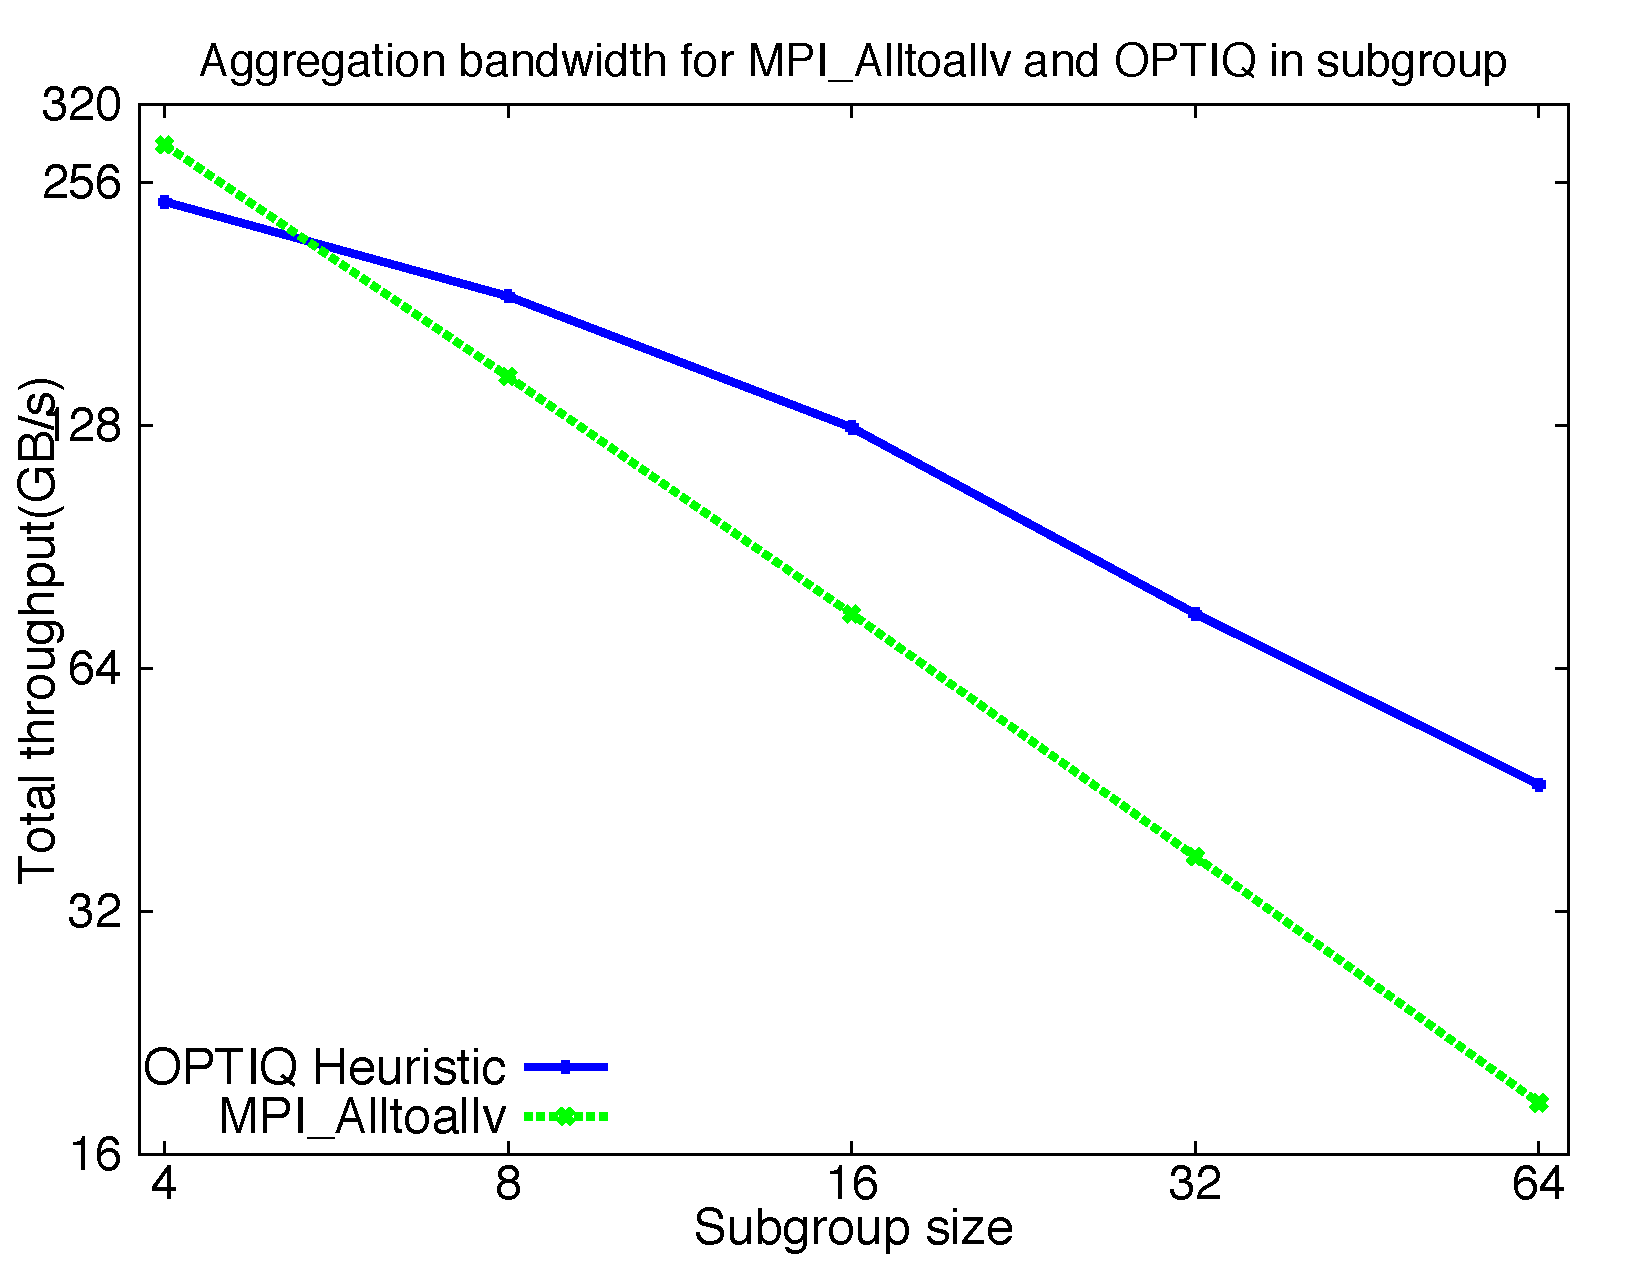
\includegraphics[scale=0.30]{figures/agg.pdf}
\vspace{-0.1in}
\caption{Aggregation bandwidth}
\vspace{-0.1in}
\label{fig:aggbw}
\end{figure}

As we can see in the figure, our work shows better performance as we increased subgroup size due to more balanced networking load. At the beginning when the size of subgroups is 4, MPI\_Alltoallv performed better. But as we doubled the subgroup size OPTIQ started to get better i.e. 1.25X at 8 nodes/subgroup, 1.7X at 16 nodes/subgroup, 2X at 32 nodes/subgroup and 2.5X at 64 nodes/subgroup. This is because OPTIQ has better network load balancing. We show the network load in the Figure \ref{fig:aggload}

\begin{figure}[!htb]
\vspace{-0.1in}
\centering
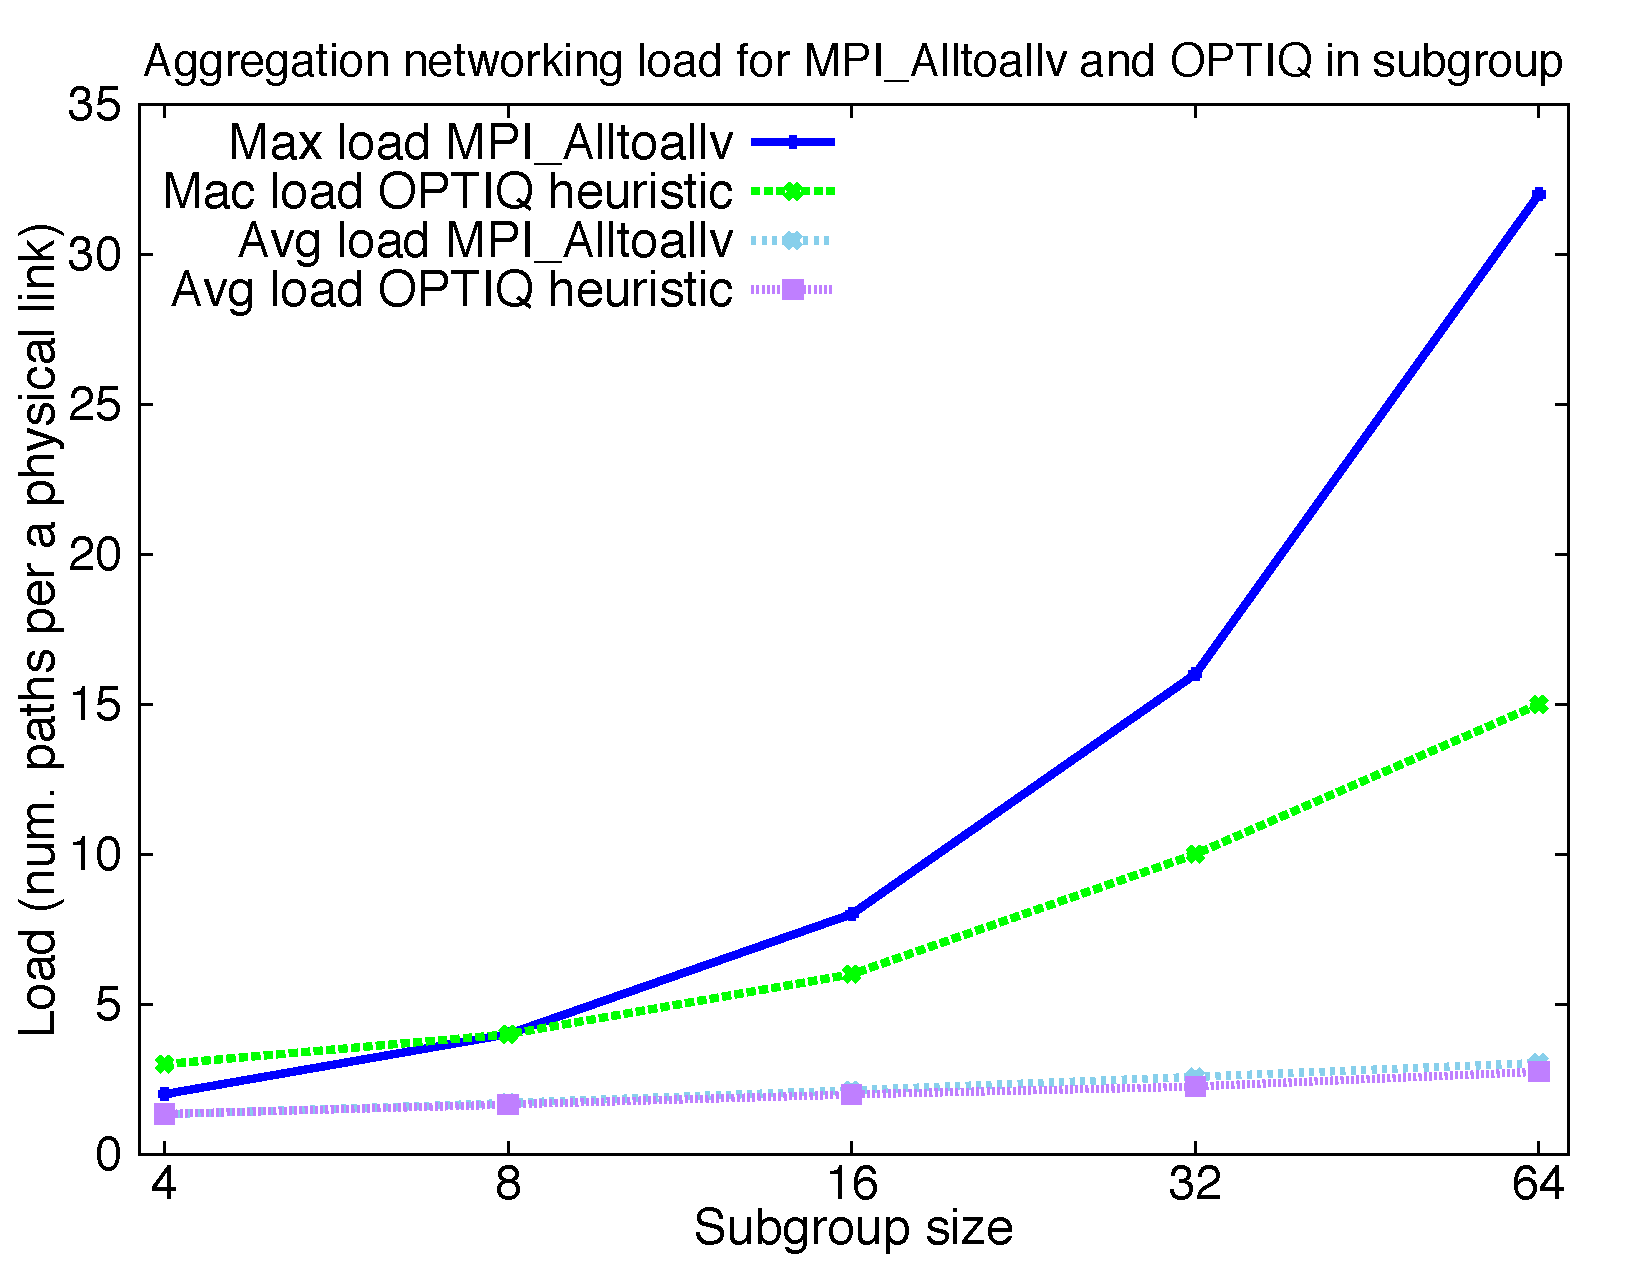
\includegraphics[scale=0.30]{figures/load.pdf}
\vspace{-0.1in}
\caption{Networking load over links}
\vspace{-0.1in}
\label{fig:aggload}
\end{figure}

Figure \ref{fig:aggload} shows the max and average loads for both MPI\_Alltoallv and OPTIQ. Load is number of paths that used a physical link. As we can see in the figure, when the group size increased the average load is approximate the same, but max load increased much faster in MPI\_Alltoallv compare to OPTIQ. This is because MPI\_Alltoallv used default routing algorithm. The default routing algorithm routes data in the longest dimension first leading to more load on certain links and no loads on many other links. Hence the max load in MPI\_Alltoallv is higher than OPTIQ. Our work distributes the networking load over more links with lower max load. The networking distribution is shown in Figure \ref{fig:aggdist}

\begin{figure}[!htb]
\vspace{-0.1in}
\centering
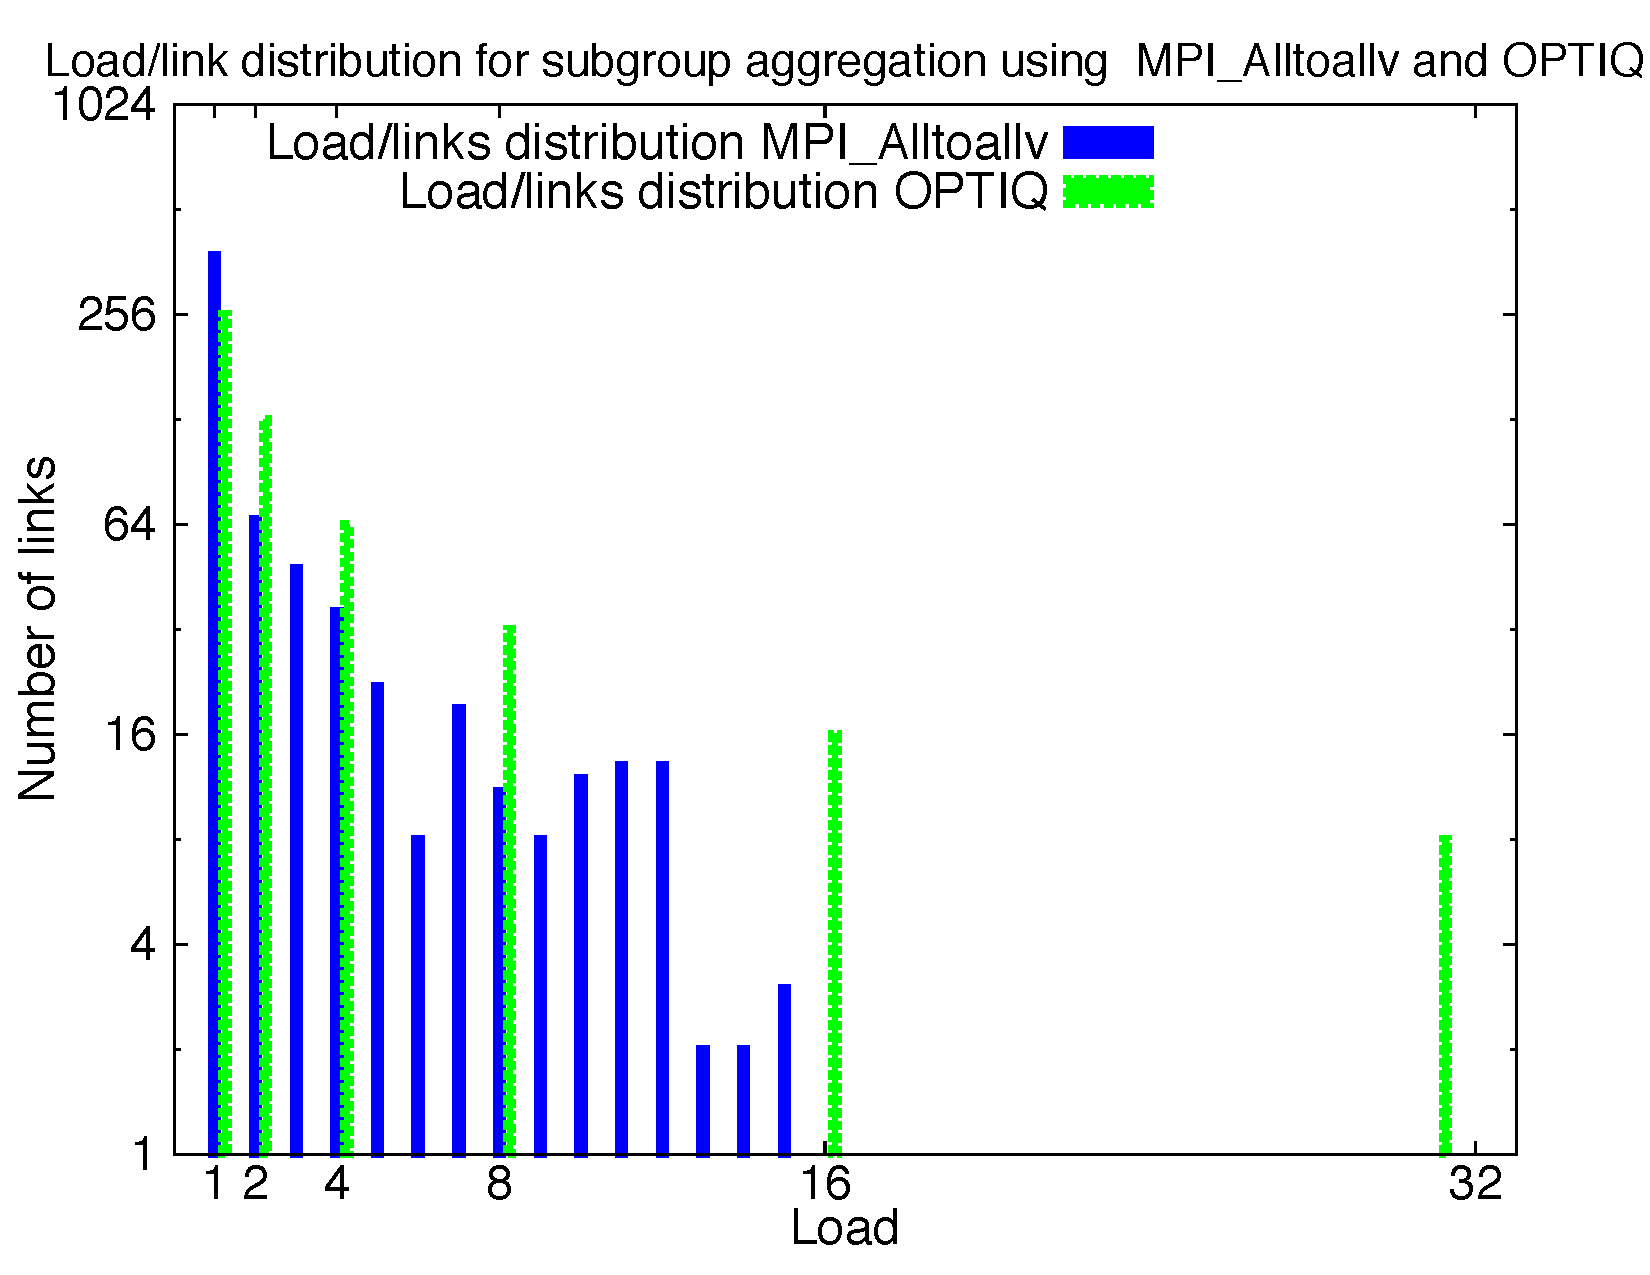
\includegraphics[scale=0.30]{figures/distribution.pdf}
\vspace{-0.1in}
\caption{Networking load distribution over links}
\vspace{-0.1in}
\label{fig:aggdist}
\end{figure}

Figure \ref{fig:aggdist} shows that our work has a better networking load distribution. All of the loaded links have max load at most of 15, with many links has low load. While MPI\_Alltoallv has 8 links with max load of 32. We achieved better load distribution by using more links and by using longer links. This leads to a little higher max hops (1 or 2 hops) and average hops used. The Figure \ref{fig:agghop} shows the maximum and average number of hops used.

\begin{figure}[!htb]
\vspace{-0.1in}
\centering
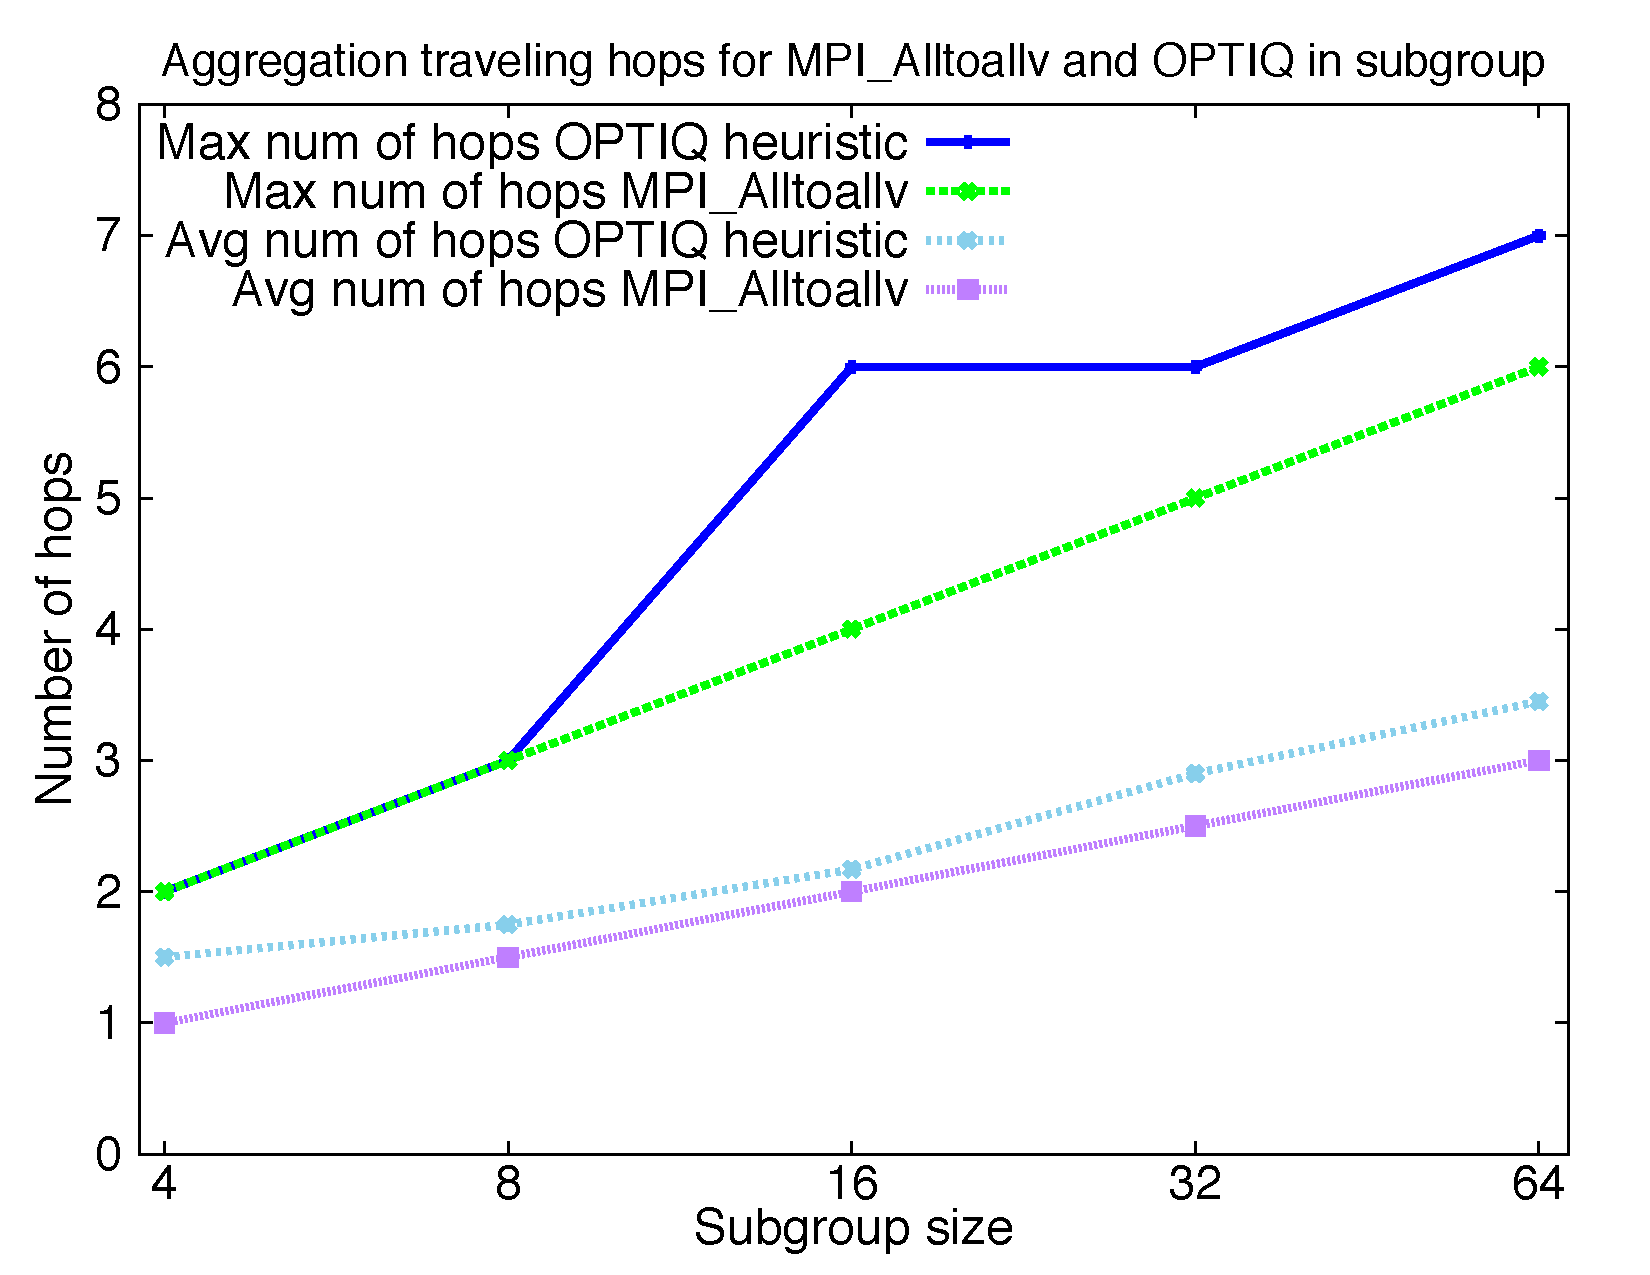
\includegraphics[scale=0.30]{figures/hop.pdf}
\vspace{-0.1in}
\caption{Max and average hops in data aggregation}
\vspace{-0.1in}
\label{fig:agghop}
\end{figure}

In the Figure \ref{fig:agghop} we can see that compare to MPI\_Alltoallv, OPTIQ used 1 to 2 hops more in case of maximum number of hops and 0.5 hops more in case of average number of hops. This is because OPTIQ explored longer paths to avoid increasing max load. The algorithms we have also try to balance between number of hops and max load as too long paths can actually increase time hence degrade data movement bandwidth.

\subsection{Scalability}
Show scalability by partition size, number of ranks per node and message sizes

\end{comment}

